\documentclass[inf, g]{pjatkThesis}
%
\usepackage{xurl}
\usepackage{float}
%\usepackage{fancyhdr}
%\pagestyle{fancy}
\usepackage{times}
\usepackage[polish,english]{babel}
%
\usepackage{sidecap}
\usepackage{graphicx}
\graphicspath{ {Images/} }
\usepackage{wrapfig}
\usepackage{subcaption}
\newcommand*{\captionsource}[2]{%
  \caption[{#1}]{%
    #1%
    \\\hspace{\linewidth}%
    {Źródło:} #2%
  }%
}
%
\usepackage{makeidx}
\usepackage{xargs} 
\usepackage{lipsum}
\usepackage[pdftex,dvipsnames]{xcolor}
%
%TODO Show \thiswillnotshow notes, remove line below for final version, and review after
\usepackage[disable,colorinlistoftodos,prependcaption,textsize=tiny]{todonotes} % use \usepackage[disable]{todonotes} to switch off
\newcommandx{\unsure}[2][1=]{\todo[linecolor=red,backgroundcolor=red!25,bordercolor=red,#1]{#2}}
\newcommandx{\info}[2][1=]{\todo[linecolor=OliveGreen,backgroundcolor=OliveGreen!25,bordercolor=OliveGreen,#1]{#2}}
\newcommandx{\change}[2][1=]{\todo[linecolor=blue,backgroundcolor=blue!25,bordercolor=blue,#1]{#2}}
\newcommandx{\improvement}[2][1=]{\todo[linecolor=Plum,backgroundcolor=Plum!25,bordercolor=Plum,#1]{#2}}
\newcommandx{\thiswillnotshow}[2][1=]{\todo[disable,#1]{#2}}
%
%
\usepackage{listings,xcolor}
%Listings settings
\lstset{
tabsize = 4, 
showstringspaces = false, %% prevent space marking in strings, string is defined as the text that is generally printed directly to the console
numbers = left, 
commentstyle = \color{green}, 
keywordstyle = \color{blue}, 
stringstyle = \color{red}, 
rulecolor = \color{black}, %% set frame color to avoid being affected by text color
basicstyle = \small \ttfamily , %% set listing font and size
breaklines = true, 
numberstyle = \tiny,
}
%
%
%

\author{Kamil Kacprzak}
\album{s14004}
% na przykładzie - gdyby było za dużo 
%Zastosowanie technologii rzeczywistości
%A+B
\title{Analiza technologii rzeczywistości rozszerzonej w biznesie ze szczególnym uwzględnieniem rękawicy-kontrolera}
\type{Praca inżynierska}
\supervisor{dr Krzysztof Barteczko}
\location{Warszawa}
\date{czerwiec 2020}
%
%
%
\begin{document}
\selectlanguage{polish} 
\begin{abstract}
%\lipsum
\end{abstract}
\selectlanguage{english} 
\begin{abstract}
%\lipsum
\end{abstract}
 
\selectlanguage{polish}
\tableofcontents
%\listoftables
\pagenumbering{arabic}
\baselineskip=22pt
\chapter{Wstęp}
\label{ch:wstep}
\change{cel i zarys, wytłumaczenie tytułu}
\chapter{Zagadnienia}
\label{ch:zagadnienia}
Aby zagłębić się w temat rozszerzonej rzeczywistości trzeba przede wszystkim zrozumieć czym jest rzeczywistość oraz zdefiniować pojęcia które są używane z tym zagadnieniem. Oprócz tego zostanie opisana historia powstania wirtualnych światów, dotycząca zarówno pierwszych urządzeń jak i wyobrażenia wirtualnego świata przez twórców filmów, a także zostanie opisany świat wirtualny z którego każdy może skorzystać i to już od wielu lat. W tym rozdziale opisano szczegółowo rozdzielenie różnych rodzajów rzeczywistości oraz na podstawie zebranych danych zostały wysunięte wnioski dotyczące potencjału technologii.

\section{Historia kreowania rzeczywistości}
\label{sec:historia}
Rzeczywistość według słownika jest to coś co istnieje naprawdę, bądź sytuacja lub warunki, w których ktoś żyje, coś się odbywa~\cite{sjp1}. Rozróżnienie tych dwóch definicji jest kluczowe ze względu rozszerzonej rzeczywistości. Rozszerzona rzeczywistość jest to tworzenie nowej formy rzeczywistości poprzez krzyżowanie obiektów rzeczywistych i cyfrowych. Z tego punktu widzenia można zauważyć że według drugiej definicji, rozszerzona rzeczywistość jest częścią rzeczywistości, w szczególności jeśli interakcja pomiędzy światami jest częścią czyjegoś codziennego życia. W przypadku pierwszej definicji, rozróżnienie jest bardziej wyraźne - to o czym mowa musi być prawdziwe, istnieć naprawdę. Z racji tego że na moment pisania tej pracy, integracja pomiędzy światami wirtualnymi oraz rzeczywistymi nie jest wystarczająco komfortowa aby mówić o użytkowaniu jej na równi z światem rzeczywistym, w dalszej części pracy jako rzeczywistość, przyjmuje się pierwszą definicje~\cite{XR}. Typy rozszerzonej rzeczywistości wraz z ich definicjami są przedstawione w sekcji~\ref{sec:rodzaje}, jednak z perspektywy historii, wszystko zaczęło się od jednego typu nazywanego wirtualną rzeczywistością - w skrócie VR (z ang. Virtual Reality). Pierwszym urządzeniem pozwalającym użytkownikowi na zajrzenie do wirtualnego świata, a konkretnie tworzenie złudzenia przebywania w innym miejscy jest Sensorama. Produkt ten został stworzony w 1962 roku przez Mortona Heiliga. Projekt ten powstał przed grafiką komputerową w związku z czym bazował na wyświetlaniu filmów jako obrazu. Zaledwie trzy lata później Ivan Sutheraland nazywany również ojcem grafiki komputerowej, pokazał maszynę do generowania wirtualnej rzeczywistości o nazwie Ultimate Display. Niestety była ona dużych rozmiarów jak i wagi, w związku z czym musiała być przymocowana do sufitu. W 1977 roku postęp technologiczny trwa, rozwijając nie tylko komputery ale także technologię VR - Dan Sandin stworzył pierwszy kontroler pozwalający użytkownikowi na interakcje ze światem wirtualnym w postaci rękawicy. Jest to początek dla projektów prezentowanych w dalszej części tej pracy. Wraz z latami osiemdziesiątymi powstały pierwsze urządzenia typu kinect, czyli pozwalające na kontrolowanie oraz interakcję ze światem przy pomocy kamery śledzącej nasze ciało. Jednak dopiero lata dziewięćdziesiąte pozwoliły na użytek technologii w stopniu wystarczającym aby nadawał się on do użytku w branży rozrywkowej. Wirtualna rzeczywistość przeżywa swój prawdziwy rozkwit po raz pierwszy, a to za sprawą powstania firm produkujących pierwsze gogle i rękawice do  wykorzystania w VR, zaprezentowaniu pierwszego urządzenia dla konsumentów którzy mogli korzystać ze swojego ciała w świecie wirtualnym przy użyciu wielu czujników oraz zakupie limitowanych zestawów, a także odkrycie potencjału przez branże rozrywkową, próbującą wprowadzić na rynek liczne produkty. Wzmożone zainteresowanie przyczyniło się również do powstania wielu filmów związanych z tym tematem co jeszcze bardziej pogłębiło zainteresowanie wśród ludzi. Wyobrażenia z filmów jednak odstają znacząco od możliwości technologicznych, a sam rozwój technologii nie jest tak szybki. Z tego oraz wielu innych powodów zainteresowanie normuje się aż do czasu pojawienia się na rynku Oculus Rift  w 2011 roku, który na nowo intryguje ludzi oraz pogłębia ogólne zainteresowanie technologią VR. Więcej na temat googli Oculus oraz innych urządzeń aktualnie znajdujących się na rynku jest powiedziane w sekcji~\ref{sec:okulary}~\cite{historia}.
  
\section{Wpływ kultury na rozwój technologii}
\label{sec:wplyw}
Od dawna wiadomo że rozwój technologii oraz kultura idą ze sobą w parze. Technologia ma wpływ na twórców oraz artystów, pozwalając im tworzyć nowe, bardziej kreatywne wizje przyszłości, jednocześnie dostarczając lepszych do tego środków, a na podstawie tej twórczości wielu naukowców bazowało się tworząc przełomowe wynalazki, takie jak samo prowadzące się samochody czy telekomunikację cyfrową. Również z technologią VR nie było inaczej. W poniższej sekcji zostanie przedstawione jak twórcy kinematografii prezentowali świat wirtualny, jakie to ma skutki na technologię z której teraz korzystają ludzie a także zostanie pokazany świat wirtualny który był dostępny zanim ludzkość odkryła elektryczność~\cite{wynalazki}.

	\subsection{Kinematografia}
	\label{subsec:kino}
	Wśród pozycji filmowych które zdecydowanie miały wpływ na postrzeganie wirtualnej rzeczywistości znajduję się kilka klasyków. Przede wszystkim warto wspomnieć o filmie \textit{Tron}, który zadebiutował w 1982 roku. Film ten pomimo fabuły ściśle powiązanej z technologią, pokazujący losy programisty przeniesionego do pamięci komputera. Kolejną ważną rolą tego filmu było szerokie zastosowanie grafiki komputerowej. W latach dziewięćdziesiątych wraz z rozpowszechnieniem się technologii, temat VR stał się dużo bardziej popularny co również można zaobserwować na podstawie tworzonych filmów. To właśnie w tym okresie powstały produkcje takie jak \textit{Johnny Mnemonic}, pokazujący możliwość przenoszenia danych przy pomocy umysłu, \textit{Kosiarz umysłów} - czyli ekranizacja powieści Stephena Kinga, w której wygenerowano komputerowo cyberprzestrzeń, pobudzając wyobrażenie zastosowania tej technologii w rzeczywistości i przede wszystkim \textit{Matrix}. Kultowa pozycja pokazująca ludzi zamkniętej w wirtualnej rzeczywistości którzy sami nie są tego świadomi z powodu realizmu który jest prezentowany - czyli dokładnie to co jest założeniem wirtualnej rzeczywistości. W filmach tych prezentuje się wiele metod łączenia umysłów wraz z technologią co nie wątpliwie było inspiracją dla wielu osób~\cite{filmy}. Z nowszych pozycji niewątpliwie należy wspomnieć o filmie \textit{Ready Player One}, który pokazuję wizję wirtualnego świata, realnego lecz jednocześnie z elementami dostępnymi tylko w środowisku wirtualnym. Film ten bazuje na wielu elementach technologicznych  dostępnych w chwili obecnej na rynku, jednak nie zintegrowanych ze sobą a przede wszystkim bez powszechnego dostępu co mogłoby pozwolić na zintegrowanie użytkowników ze światem wirtualnym. Jest on dla wielu wizją tego w jakim kierunku zmierza technologia oraz integracja wielu urządzeń takich jak bieżnie pozwalające na przemieszczanie się w każdym kierunku, realna odczucia całego ciała przy wykorzystaniu odpowiednich kombinezonów no i oczywiście kontrola oraz interakcja przy wykorzystaniu rękawic oraz ciała użytkownika~\cite{p1}. Wszystkie te wizje sprawiają że użytkownicy pragną coraz bardziej realnych doznań oraz interakcji, a także możliwości osiągnięcia wykonania zadania bez konieczności wychodzenia z domu. Oczywiście realizując to, każdy wie że znajduje się w świecie wirtualnym z powodu świadomego przejścia. Gdyby jednak nawet ktoś się obudził w takiej przestrzeni nieświadomy tranzycji pomiędzy rzeczywistościami, łatwo można to określić na podstawie zamontowanych kontrolerów, kombinezonów czy okularów które wyczuwa się na ciele, a także wad elementów graficznych którym wciąż brakuje wystarczającego realizmu. Istnieje jednak metoda która pozwala temu zapobiec, która może posłużyć jako przykład wirtualnego świata w trybie pojedynczego gracza.
	
	\subsection{Marzenia senne}
	\label{subsec:sny}
	Podczas analizy sztucznej rzeczywistości ważnym punktem jest sen, a konkretnie marzenia senne. Przeciętnie człowiek potrzebuje od siedmiu do dziewięciu godzin snu dziennie w cyklu monofazowym, czyli gdy zasypia się i budzi tylko raz dziennie. W tym czasie występują marzenia senna, potocznie nazywane snami. W zależności od osoby swoje sny można pamiętać bądź nie, jednak warto podkreślić że każda osoba ma sny - zapamiętywanie marzeń sennych, tak jak z każdą inną umiejętność można wytrenować, aby pamiętać więcej szczegółów, miejsc oraz wydarzeń. Mając to na uwadze należy sprecyzować czym one właściwie są. Marzenia senne są serią myśli, obrazów oraz odczuć które dana osoba przeżywa w swoim umyśle w trakcie snu. Nie jest to też dowolny moment w trakcie spania. Sen odbywa się w cyklach, które średnio trwają dziewięćdziesiąt minut i składają się z kilku faz takich jak sen przejściowy, głęboki sen czy faza ruchu gałek ocznych - w każdej fazie można śnić jednak to w tej ostatniej najczęściej występują marzenia senne które są rzeczywiste i realistyczne - w wielu przypadkach nie sposób ich odróżnić od rzeczywistości. Faza ta nazywana fazą REM ( z ang. Rapid Eye Movement) jest etapem snu w którym nasz umysł wprowadzany jest w specjalny stan aby móc osiągnąć ten efekt. Przede wszystkim warto zauważyć że etap ten charakteryzuje się wysoką aktywnością mózgu, porównywalną z tą gdy osoba jest przytomna, sprawia to że bardzo łatwo przerwać ten etap i wybudzić się w trakcie snu. Oprócz tego w naszym mózgu przepływa wiele impulsów przez różne jego obszary, niejako testując połączenia, co jest podejrzewane jako przyczynę tworzenia się w naszym umyśle obrazów, doznań dźwiękowych oraz ruchowych. Aby jednak impulsy nie zostały wysłane do mięśni w ciele, w trakcie snu występują ich atonia, czyli zniesienia napięcia mięśniowego. W ten sposób w trakcie gdy ciało leży nieruchomo, w odpowiednim momencie snu dochodzi do symulacji świata w umyśle, w trakcie której osoba może przeżywać wydarzenia które mogą być nawet nie możliwe do zrealizowania w świecie rzeczywistym. Interesującym jest więc fakt, że większość osób zdaje sobie sprawę tuż po przebudzeniu, że wydarzenia które przed chwilą miały miejsce były jedynie marzeniami sennymi - nie były one rzeczywistością. Dzieje się tak za sprawą kory przedczołowej - części mózgu która jest odpowiedzialna za myślenie logiczne, planowanie ruchów i działań, oraz pełni funkcje w działaniu pamięci roboczej. Kora przedczołowa jest jednym z obszarów mózgu który w trakcie snu wytwarza jedynie minimalną aktywność co sprawia że gdy marzenia senne zaczynają się w zupełnie innym miejscu od lokalizacji danej osoby, z ludźmi których dana osoba nie zna, bądź wręcz nie powinno ich tam być, jak na przykład osoby zmarłe bądź znajdujące się w innym miejscu na ziemi, mózg tego nie kwestionuje - przyjmuje że to co się dzieje jest zupełnie normalne. Za sprawą tych mechanizmów, niejako każda osoba codziennie ma dostęp to sztucznej rzeczywistości w której może znaleźć się w dowolnym miejscu, z dowolnymi osobami, przeżywając zdarzenia które mogą być nawet sprzeczne z prawami fizyki. 
	
W obecnych czasach jeżeli mówimy o wirtualnej rzeczywistości, nie myślimy o maszynie takiej jak Sensorama, która jedynie wyświetlała filmy. Poruszając ten temat myślimy o kontrolowanym środowisku w którym użytkownik ma możliwość interakcji z otoczeniem a nawet jego kontrole. W rozumieniu marzeń sennych, zwykłe sny są tym czym Sensoroma jest dla współczesnej technologii VR. Świadome śnienie natomiast odkrywa pełną moc możliwości która kryje się w tym naturalnym ludzkim procesie. Aby podjąć próbę świadomego snu należy oczywiście najpierw być w stanie pamiętać swoje zwyczajne marzenia senne. Świadomy sen jest to rodzaj snu w którym osoba śniąca zdaje sobie sprawę z tego że znajduje się w świecie marzenia sennego. Istnieje wiele metod które pozwalają osiągnąć ten stan, jednak ogólnie mówiąc sprowadzają się one do kwestionowania rzeczywistości, dzięki czemu możemy niejako zakodować ten proces w podświadomości. Tak jak wspomniano kora przedczołowa odpowiadająca za logiczne myślenie nie wykazuje dużej aktywności w trakcie snu, jednak nie jest ona całkowicie nieaktywna, dzięki czemu nadal można ją wykorzystać nawet podczas snu. Jeżeli osoba zakwestionuje rzeczywistość w trakcie marzenia sennego, na przykład poprzez złamanie praw fizyki, i rezultat takiego testu pokaże niemożliwe rezultaty w świecie rzeczywistym, osoba taka odzyskuje świadomość. Często w początkowych próbach dochodzi w tym momencie do wybudzenia, ponieważ jest to niejako przełamanie naturalnego mechanizmu organizmu. Z praktyką jednak dochodzi do stabilizacji świata a dzięki uzyskaniu świadomości, dochodzi do uzyskania kontroli nad naszym umysłem, czyli marzeniem sennym. W ten oto sposób mózg od wewnątrz, bez dodatkowych urządzeń i kontrolerów, generuje własny świat ''wirtualny``, odtwarzając bodźce wzrokowe, słuchowe, dotyku oraz wszystkie inne zmysły. Osoba kontrolująca ma pełną kontrole nad własnym ciałem i z jej perspektywy świat w którym się znajduje dostarcza tych samych bodźców co świat rzeczywisty, a dla osób które potrafią kontrolować otoczenie, bodźców możliwych do doświadczenia jedynie poza światem rzeczywistym takich jak np. latanie czy teleportacja~\cite{sen2}~\cite{sen1}. 		
	
\section{Rodzaje rzeczywistości}
\label{sec:rodzaje}
Umiejętność świadomego snu jest treningiem przejęcia kontroli nad naturalnym procesem śnienia występującym u każdej osoby, pozwalając niejako doświadczyć tego dokąd technologia wirtualnej rzeczywistości zmierza - bezbłędnego odwzorowania świata rzeczywistego, przy dostarczeniu do mózgu wszystkich bodźców w taki sposób aby osoba użytkująca odniosła pełne wrażenie realizmu otoczenia. Mając to na uwadze, w tej sekcji zostanie zdefiniowane czym jest rozszerzona rzeczywistość, jakie rodzaje rzeczywistości obejmuje ten termin oraz wyjaśnić dokładnie pojęcie wirtualnej rzeczywistości które było używane w tym rozdziale. 
	%\subsection{XR}
%	\label{subsec:xr}

	Akronim XR (z ang. Extended Reality) jest tłumaczony na język polski na wiele sposobów takich jak rzeczywistość rozszerzona ( w odróżnieniu od rozszerzonej rzeczywistości) czy rzeczywistość skrzyżowana. W praktyce jednak najczęściej używa się skrótów angielskich które pozwalają jednoznacznie określić zagadnienie. Termin XR jest używany jako ogólne wyrażenie wszystkich technologii wpływających na zmianę rzeczywistości, które mogą zostać użyte razem bądź pojedynczo. W związku z tym aplikacje mieszające obiekty wirtualne z rzeczywistymi które mogą dowolnie przełączać się pomiędzy tym światem a światem czysto wirtualnym są określane tym terminem, jak i każdy z projektów wykorzystujących tylko jeden typ technologii zmiany rzeczywistości. W chwili pisania tej pracy terminem XR określa się zbiór technologi wirtualnej rzeczywistości, rozszerzonej rzeczywistości a także mieszanej rzeczywistości, jednak określenie to powstało w celu włączenia do jednego określenia również wszystkich terminów które mogą zostać stworzone w przyszłości~\cite{terms}.
	%\subsection{VR}
	%\label{subsec:vr}
	
	Pojęcie wirtualnej rzeczywistości określa się skrótem VR ( z ang. Virtual Reality) i definiuje ono część technologii kreowania rzeczywistości w pełni wirtualnej - oznacza to że nie znajdują się w niej żadne elementy świata rzeczywistego. Jeżeli elementy te miały by być prezentowane w takim środowisku muszą one zostać wygenerowane komputerowo. Celem VR jest stworzenie jak najbardziej realistycznych i rzeczywistych odczuć dla użytkownika niezależnie od środowiska w jakim się znajduje. Aby to osiągnąć niezbędna jest symulacja która wpływa na wszystkie zmysły użytkownika. Dlatego też firmy pracują nad coraz bardziej realistycznymi i dokładnymi rozwiązaniami które pozwalają na głębszą imersję w świat wirtualny. Jest to również jednym z głównych powodów dla których zostały stworzone rękawice-kontrolery. Pozwalają one na większą swobodę oraz bardziej naturalny ruch w  wygenerowanej przestrzeni, zapewniając lepsze odczucia oraz komfort podczas przebywania w świecie wirtualnym. Nad zapewnieniem realizmu, oprócz metody kontroli środowiska, składa się wiele innych czynników. W tym celu powstają specjalne kombinezony które odwzorowują ruch całego ciała, bieżnie które pozwalają się poruszać w VR, dzięki naturalnemu przemieszczeniu się, które za sprawą bieżni odbywa się w miejscu w świecie rzeczywistym, okularów które pozwalają wyświetlać przed oczami środowisko wirtualne, starając się odwzorować głębię oraz wiele innych urządzeń. Ilość urządzeń oraz metod imitacji pokazuje jak skomplikowanym problemem jest odwzorowanie rzeczywistości, a wszystko to musi odbywać się niezwykle płynnie ponieważ mózg człowieka nie rozróżnia rzeczywistości od świata wirtualnego. Oznacza to że jeżeli bodźce wzrokowe nie pokrywają się z bodźcami słuchowymi dochodzi do tak zwanego zjawiska choroby lokomocyjnej. Sprawia to że przebywania w wirtualnym świecie przez długi okres czasu może doprowadzić do dyskomfortu dla użytkownika. Aby zapobiec tego rodzaju problemom równie ważnym jest dokładna znajomość fizjologii człowieka, co prowadzi do współpracy wielu działów nauki w celu stworzenia prawdziwie realistycznych produktów. Pomimo wielu przeszkód jak przedstawiono w sekcji~\ref{sec:historia}, wirtualna rzeczywistość była pierwszą wizją naukowców którą starano się zrealizować - pomimo dużych nakładów pracy w celu zapewnienia realistyczności, niesie ona za sobą wiele możliwości zarówno w biznesie jak i życiu codziennym, co sprawia że dla wielu firm jest to możliwość realizowania własnej wizji wirtualnej przyszłości~\cite{terms}~\cite{chorobaVR}.
	%\subsection{AR}
	%\label{subsec:ar}
	
	Kolejnym terminem wchodzącym w skład XR jest rozszerzona rzeczywistość, bądź też nazywana rzeczywistością poszerzoną. Skrótowo zapisuje się ją jako AR (z ang. Augmented Reality). Podobnie brzmiąca do XR w szczególności w języku polskim jest częstym powodem dla którego powszechnie używa się skrótów angielskich mówiąc o tym obszarze technologii. AR jak nazwa wskazuje poszerza rzeczywistość zamiast ją zastępować tak jak to miało w przypadku VR. Oznacza to że do elementów świata rzeczywistego zazwyczaj pozyskanych przy pomocy obrazu z kamery, wyświetlanych poprzez wybrane źródło obrazu o których mowa w rozdziale~\ref{ch:prezentacja}, są dodawane elementy stworzone przy pomocy grafiki komputerowej, zazwyczaj trójwymiarowe. Technologia ta dzięki wykorzystaniu w dużej mierze świata rzeczywistego jest łatwiejsza w użytkowaniu a jej zastosowanie jest powszechnie stosowane w wielu branżach. W szczególności duży sukces technologia ta odniosła gdy wykorzystano ją do stworzenia popularnej gry na smart-fony \textit{Pokemon Go}, która przy wykorzystaniu geolokalizacji oraz AR zapewniała realistyczne doświadczenia łapania stworzonych trójwymiarowych postaci w świecie rzeczywistym~\cite{terms}. Podgląd interfejsu aplikacji obrazujący wykorzystanie technologii AR  w \textit{Pokemon Go} pokazuje rysunek~\ref{fig:pokemon}.
	
\begin{figure}[h]
\centering
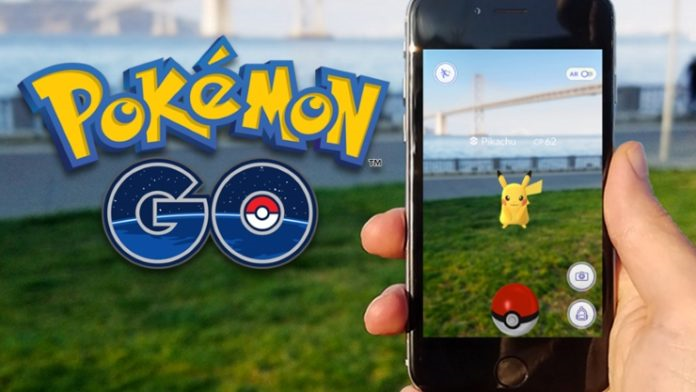
\includegraphics[scale=0.6]{pokemon}
\captionsource{Interfejs aplikacji \textit{Pokemon Go} wykorzystujący AR.}{\url{https://gameradar.pl/aktualizacja-pokemon-go-utrudnia-lapanie-pokemonow/}}
\label{fig:pokemon}
\end{figure}

	%\subsection{MR}
	%\label{subsec:mr}	
	
	Mieszana rzeczywistość, czyli MR (z ang. Mixed Reality) jest terminem który prawdopodobnie jest najczęściej błędnie używanym wśród zagadnień związanych z XR. Mieszana rzeczywistość podobnie jak AR wykorzystuje do działania zarówno świat rzeczywisty jak i stworzony komputerowo, jednak w odróżnieniu od AR nastawiony jest głównie na interakcję pomiędzy tymi światami. Obiekty tworzone cyfrowo wyświetlane w świecie rzeczywistym mogą być modyfikowane i wpływać na środowisko rzeczywiste które jest wyświetlane jak i obiekty rzeczywiste mogą zostać przeniesione do świata wirtualnego. Interakcja ta i zastosowanie jest niejako technologią przyszłości, wizją producentów, ponieważ do tej pory nie ma łatwo dostępnych produktów które by wykorzystywało ten rodzaj XR, natomiast istnieją takie rozwiązania dla biznesu oraz w ośrodkach badawczych, które prawdopodobnie staną sie bardziej dostępne wraz z rozwojem tej technologii oraz ulepszonych rozwiązań w innych dziedzinach technologicznych takich jak grafika komputerowa, prędkość przesyłania czy przetwarzania danych~\cite{terms}.
%\section{Potencjał technologii}
%\label{sec:potencjal}

Rozwiązania XR przebyły długą drogę od czasu powstania pierwszej wizji tego typu rozwiązania. Obecnie istnieje wiele urządzeń które powszechnie korzystają z XR zarówno na użytek prywatny, branży rozrywkowej oraz w celu usprawnienia procesów biznesowych. Niemniej jednak dopiero są opracowywane rozwiązania które mogłyby zapewnić większą przenośność tego typu urządzeń, sprawniejsze połączenie i przede wszystkim realizm. Wykorzystanie w życiu codziennym staje się coraz bardziej powszechne, w związku z tym można też się  spodziewać ulepszeń produktów zarówno pod względem sprzętu jak i oprogramowania a także dostępności tych produktów przy mniejszym koszcie. Można być pewnym że technologia ta nie przestanie się rozwijać, znajdując coraz to nowe zastosowania, inwestorów a także twórców którzy wprowadzając większą liczbę produktów na rynek, tworzą większe zainteresowanie wśród społeczności. Pytanie stawiane przez technologię XR to nie czy ta technologia ma przyszłość, a kiedy stanie się ona powszechnie stosowana. W dalszych częściach tej pracy zostaną pokazane sposoby w jakich obecnie przedstawiane i wykorzystywane są opisywana do tej pory technologie, a także zostanie szczegółowo opisany temat rękawic-kontrolerów, urządzenia które nie jest standardem wśród kontrolerów na rynku dla pojedynczych konsumentów VR, jednak już jest wykorzystywany w biznesie a także przewidywany jest jako kontroler przyszłości~\cite{terms}.


\chapter{Interakcja z kreowaną rzeczywistością}
\label{ch:prezentacja}

\section{Okulary VR}
\label{sec:okulary}

\section{Smart-fon jako urządzenie do prezentacji}
\label{sec:smartphone}

\section{Kontrolery i IoT}
\label{sec:iot}

	\subsection{Problemy kontrolerów}
	\label{subsec:problemy}
	
	\subsection{Działanie czujników}
	\label{subsec:dzialanie}
	\change {IMU}
\section{Dłoń jako kontroler}
\label{sec:dlon}
% przejscie do nastepnego rozdzialu

\chapter{Rękawice jako kontrolery}
\label{ch:kontrolery}
Kontroler w postaci rękawicy jest pojęciem często używanym ze względu na popularność tego rozwiązania. Rękawiczka zakładana na dłoń z zamontowanymi czujnikami dzięki którym deweloper uzyskuje wszelkie potrzebne informacja aby wchodzić w interakcję z otoczeniem. Idea która za tym stoi nie dotyczy jednak rękawiczki samej w sobie - chodzi o wykorzystanie ludzkiej dłoni jako kontrolera a rękawiczka jest używana jako nośnik temu służący. Ze względu na różne podejścia istnieją typy kontrolerów wykorzystujących dłoń do obsługi świata, które zostaną opisane w dalszej części tego rozdziału. Kontrolery a w szczególności dłonie są głównie wykorzystywane w świecie VR, w pozostałych rodzajach XR wystarczyłaby analiza obrazu na podstawie której określa się interakcję użytkownika z otoczeniem. W przypadku VR które przenosi użytkownika do zupełnie innego świata, wykorzystanie kontrolerów wydaję się więc obowiązkowe.  
\section{Rozwój rękawicy jako kontrolera}
\label{sec:rozwojVR}
	Pomysł wykorzystania dłoni jako kontrolera, pomimo wielu lat od pierwszego wdrożenia wciąż znajduje zastosowania głównie w biznesie, jednak produkty te są dostępne również dla zwykłych konsumentów. Problemem jest jednak cena która czasami wynosi tyle co zestaw do obsługi VR bądź więcej. Oprócz tego nie ma zbyt wielu pozycji w sklepie które by wykorzystywały w sposób szczególny tego rodzaju kontrolery. Dlatego też to właśnie głownie firmy są zainteresowane tego typu produktami, które dla specyficznego przypadku tworzą aplikacje obsługujące tego typu kontrolery. Wykorzystanie XR i rękawic kontrolerów w biznesie pokazano w rozdziale~\ref{ch:biznes}. Jednak aby produkt ten był w stanie spełnić oczekiwania rynku musiał przejść długą drogę od projektu stworzonego przez Dana Sandina. Jego rękawica \textit{The Sayre Glove} była w pełni przewodowa a jedynymi czujnikami które obsługiwała był pomiar wygięcia palców, służący głównie do zmiany pozycji suwaków. Była jednak tania i lekka co spełniało podstawowe oczekiwania w tamtych czasach. Rękawice tą przedstawia rysunek~\ref{fig:sayra}.
\begin{figure}[h]
\centering
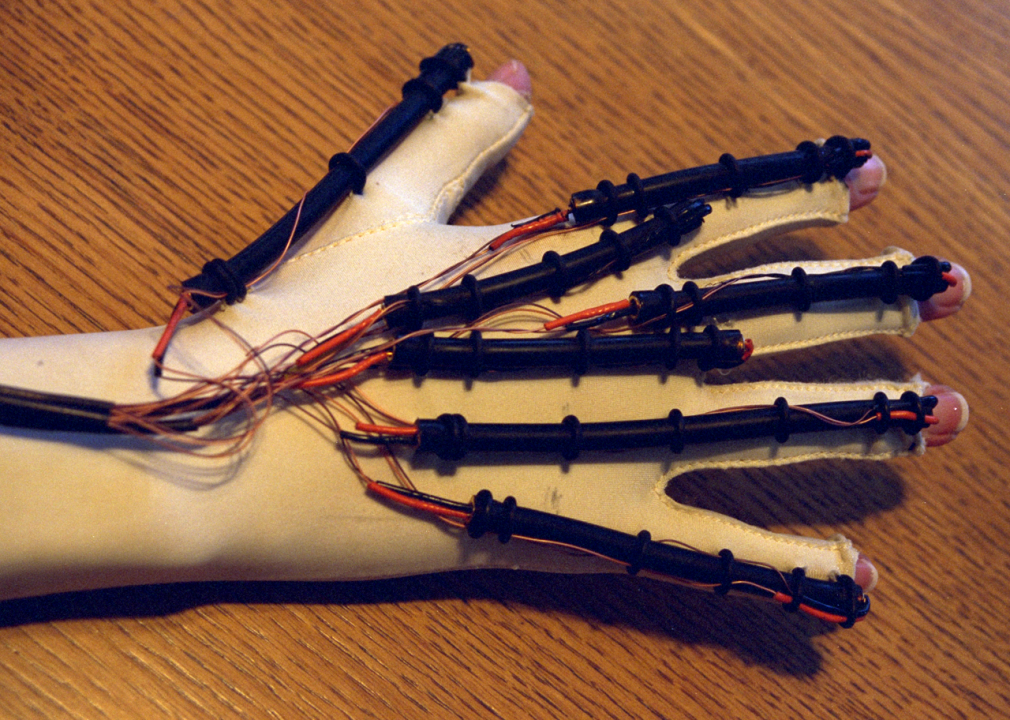
\includegraphics[width = 0.7\textwidth]{sayra}
\captionsource{Pierwsza rękawica VR - Sayra Glove}{\url{https://www.evl.uic.edu/entry.php?id=2162}}
\label{fig:sayra}
\end{figure}
W 1983 roku Gary Grimes stworzył kolejny produkt warty uwagi - była to rękawica która potrafiła rozpoznawać osiemdziesiąt specjalnych gestów, które następnie były zamieniane na litery alfabetu. Produkt ten jednak nie został nigdy dostępny do kupienia. Kilka lat później, w 1987 roku nastąpił przełom w dziedzinie rękawic kontrolerów. Została stworzona rękawica która potrafiła monitorować sześć stopni swobody - oznacza to przemieszczenie oraz orientację wokół trójwymiarowego układu współrzędnych. Wykonana została przez Thomasa Zimmermana wraz ze współpracownikami i została spopularyzowana i rozpowszechniona na całym świecie. Niewątpliwie był to największy przeskok w rozwoju tego urządzenia od czasu pierwszego projektu. Dwa lata później powstała rękawica która jako pierwsza była dostępna w celach rozrywkowych. Stworzona przez firmę zabawkową Mattel, dla gier konsolowych produkowanych przez Nintendo, rękawica nazwana \textit{The Power Glove}. Produkcja jednak została przerwana po dwóch latach od wprowadzenia na rynek produktu. Są to wybrane pozycje które w jakimś stopniu zmieniły rynek oraz wprowadziły zmiany w tym segmencie. Wraz z dalszym rozwojem wirtualnej rzeczywistości powstały kolejne produkty a w szczególności po roku 2000, podczas pierwszej fali popularności technologii VR powstało wiele dopracowanych produktów~\cite{ewolucja}. 
\section{Podział rękawic-kontrolerów}
\label{sec:podzial}
Rozwój rękawic-kontrolerów wprowadził wiele zmian począwszy od technologii na której bazują, połączeń które używają jak i funkcjonalności które są w stanie zapewnić. Na tej podstawie nadal większość produktów stara się wyróżnić na tle konkurencji jednak bazowe podejście do produktu sprawia że można go podzielić według ogólnych kategorii, do których można zaliczyć rękawice klasyczne, systemy nasadowe oraz egzoszkielety. W dalszych częściach tej sekcji zostaną opisane szczegółowo te typy wraz z prezentacją współczesnych rozwiązań które są dostępne na rynku~\cite{review}. 

	\subsection{Klasyczne}
	\label{subsec:klasyczne}
	Pierwsze, najstarsze typy rękawic określane są jako klasyczne ponieważ przypominają one zwykłe rękawiczki używane w życiu codziennym z tym że podpięto do nich różnego rodzaju sensory, mikrokontrolery, przekaźniki danych i baterie. Innymi słowy sprawiono że zwykła rękawiczka jest w stanie zbierać dane na temat położenia dłoni i palców użytkownika, a następnie bezprzewodowo przesłać te dane do odbiornika, zapewniając przy tym wygodę pracy oraz ponad kilka godzin użytkowania na jednym ładowaniu w zależności od produktu. Prawdopodobnie najbardziej znanym produktem na rynku są rękawice należące do firmy Manus Vr, która dostarcza kilka rozwiązań w zależności od dodatku za które użytkownik chce dopłacić. Wykonane z elastycznego materiału, lekkie i cienkie dzięki czemu są przyjemne w używaniu, z materiałem odciętym w czubkach palców dla większej wygody. Waga to około 70 gramów, co sprawia że użytkowanie to czysta przyjemność. Rękawice łączą się z takimi zestawami VR jak Oculus czy Vive i są szeroko wykorzystywane na rynku biznesowym przez takie firmy jak Audi, BMW, Ubisoft czy NASA. Cena za rękawice to od 3000 do 4000 euro - zdecydowanie nie należą one do najtańszych. Od strony technicznej, w początkowej wersji tego projektu zostały zastosowane czujniki oporu, które zwracały różny opór, jednak zastąpiono je w nowszej wersji zestawem  czujników zaprojektowane przez firmę Bosch w skład których wchodzą jedenaście czujników na palcach, dwa na każdym poza kciukiem gdzie znajdują się trzy - żyroskop, akcelerometr i magnetometr dla dokładnego mierzenia położenia naszej dłoni. Czujniki te są elastyczne i działają analogowo sprawdzając knykcie oraz pierwszy staw palca a także od knykci do drugiego stawu palca łącznie dając dziesięć stref pomiaru. Czujniki orientacyjne znajdują się na wierzchniej części dłoni oraz kciuka - pomiar jest dokonywany dzięki płytce IMU zapewniającej jedenaście stopni swobody. Czujniki na palcach wskazują dokładność $\pm 3$ stopni. System śledzenia natomiast oblicza pozycję dłoni w przestrzeni dzięki użyciu innych systemów takich jak Xsens, Vive Tracking, OptiTrack, Vicon czy ART. Obsługują one pracę wielu użytkowników jednocześnie w jednym świecie wirtualnym. Bateria została wyprodukowana przez firmę Varta a producent szacuję czas pracy na baterii pomiędzy 4 a 6 godzinami intensywnego użytkowania. Rękawice działają bezprzewodowo przy opóźnieniu poniżej 5 milisekund. Wspierają one również technologię wibracji, dzięki czemu można samodzielnie zaprogramować moduł wibrujący dla odpowiednich czynności świata wirtualnego. Firma wypuściła własne wtyczki dla takich środowisk jak Unity, Unreal Engine oraz Autodesk MotionBuilder. Jest to jedno z najbardziej rozbudowanych rozwiązań na rynku które wspiera rozwój swojego oprogramowania na wielu platformach i stanowi jednego z największych konkurentów dla pozostałych produktów~\cite{manus}. Rękawice te widoczne są na rysunku~\ref{fig:manus}. Podobnym produktem występującym na rynku są rękawice firmy Noitom o nazwie \textit{Hi5}. Rękawice te kosztują znacznie mniej, ich cena to około 1000\$, jednak posiadają znacznie wiecej wad. Przede wszystkim nie wspierają one zestawu Oculus Rift. Tak jak w poprzednim przypadku, bazują one na kontrolerach ruchu dostarczonych przez zewnętrzną firmę - w tym przypadku są to kontrolery Vive. Źródłem zasilania są zwykłe baterie AA co stanowi poważny problem dla dłuższego użytkowania. Rękawice wspierają \textit{Haptic Feedback}, czyli system wibracji oparty na interakcji z przedmiotami w świecie wirtualnym, zapewniają śledzenie wszystkich palców u dłoni oraz używają czujników takich jak żyroskop, akcelerometr i magnetometr wbudowanych w jednostkę IMU. Widać więc że spełniają one stawiane przed tymi kontrolerami oczekiwania jednak posiada wiele niedociągnięć które potencjalnie zniechęcają do kupna tego produktu~\cite{hi5}. Rysunek~\ref{fig:hi5} przedstawia omawiany kontroler.
\begin{figure}[h]
\centering
	\begin{subfigure}[b]{0.4\textwidth}
	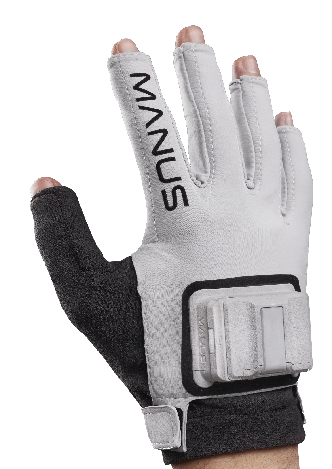
\includegraphics[width=\textwidth]{manus}
	\captionsource{Rękawica firmy Manus Vr}{\url{https://manus-vr.com/mocapgloves}\\}
	\label{fig:manus}
	\end{subfigure}
	\hspace{0.5cm}
	\begin{subfigure}[b]{0.34\textwidth}
	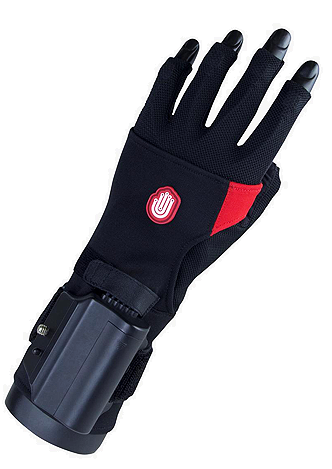
\includegraphics[width=\textwidth]{hi5}
	\captionsource{Rękawica firmy Noitom}{\url{https://hi5vrglove.com/store/hi5glove}}
	\label{fig:hi5}
	\end{subfigure}
\caption{Przykładowe klasyczne rękawice VR.}
\label{fig:rekawice}
\end{figure}	
Kolejnym produktem jest \textit{Exoglobe}, który wyróżnia się na tle konkurencji dzięki zastosowania technologii ultradźwięków. W ten sposób śledzi dłoń w prawie $180^o$ z dokładnością nawet do 0,5 mm. W oprogramowaniu rękawic znajduję się moduł sztucznej inteligencji który uczy się gestów, sposobu poruszania się oraz obszaru w którym porusza się użytkownik. Wszystko zapewniane jest za cenę 99\$ która jest zdecydowanie mniejsza od propozycji konkurencji~\cite{exo}. Avatar VR jest to produkt hiszpańskiej firmy NeuroDigital, która stworzyła rękawicę wspierającą haptic feedback, wykonaną z oddychającego materiału który również jest materiałem przewodzącym co pozwoliło zaimplementować sterowanie gestami. Za cenę 1500\$ dostajemy parę rękawiczek wraz z odbiornikiem USB który łączy się poprzez Bluetooth 4.0. Produkt zapewnia od sześciu do ośmiu godzin pracy na baterii po której należy naładować akumulator poprzez 5 V micro USB. Do rękawiczek można podłączyć odpowiednie czujniki które należy podpiąć na ramieniu oraz klatce co zapewnia śledzenie całej górnej części ciała. Sterowanie zapewniane jest poprzez 9 osiowe IMU. Rękawiczki mają wbudowanych 10 płytek wibrujących które zapewniają 1024 różnych poziomów wibracji. W rękawiczkach znajdują się 4 strefy przewodzące (dłoń, kciuk, palec wskazujący oraz środkowy). Produkt posiada również technologię NZDE (z ang. Near zero drift Experience), która pozwala powtarzać te same gesty w celu eksperymentowania w środowisku wirtualnym bez wprowadzania kumulacji znaczących błędów które gromadzą się w szczególności przy korzystaniu z danych żyroskopu~\cite{avatar}. Ostatnim produktem z kategorii klasycznych rękawic który warto wymienić są rękawice CaptoGlove. Firma produkująca ten kontroler rozszerza swoją funkcjonalność poza świat VR. Producent daje możliwość używania swoich rękawic poprzez technologię plug and play (z ang. podłącz i używaj) z komputerami oraz smart-fonami. Dzięki użyciu zapewnianego sdk można dalej przenieść nasze doświadczenia na platformy VR, konsole do gier czy kontrolować przy ich użyciu drony, roboty czy telewizory. Za pojedynczą rękawice klient zapłaci 250\$ za parę natomiast 490\$. Aby używać produktu w VR, grach wideo czy na smart urządzeniach należy dokupić Capto sensor czyli czujnik ruchu pozwalający określić położenie dłoni w przestrzeni kosztujący dodatkowe 190\$. Urządzenia kontrolujemy przy użyciu gestów dłoni, odpowiednie ruchy są tłumaczone na akcji wykonywane na różnych platformach. Na czubkach palców został umieszczony materiał pozwalający kontrolować ekrany dotykowe bez zdejmowania kontrolera. Rękawica łączy się z wymienionymi urządzeniami przy pomocy Bluetooth i według producenta pozwala na pracę przez około 10 godzin. Jest to kolejna pozycja wśród rękawic ciesząca się popularnością i jest wykorzystywana przez takie firmy i organizacje jak Mitsubishi, U.S. Air Force czy Fujitsu~\cite{capto}.  
	
	\subsection{Nasadowe}
	\label{subsec:nasadowe}
	Kolejnym typem urządzeń pozwalających na używanie dłoni jako kontrolera są urządzenia nasadowe. Nie są to typowe rękawiczki, a jedynie jej elementy których można by się spodziewać na czubkach palców, nadgarstkach czy też dłoni, które połączone odpowiednio ze sobą pozwalają na odczytywanie danych dotyczących położenia i orientacji  dłoni, palców, zapewniają wibracją oraz innego rodzaju imitacje świata rzeczywistego. W tym segmencie zdecydowanie wyróżniają się nakładki na palce, które skupiają się na symulacji dotyku, a w szczególności dwie firmy które się tym zajmują - Tactai z nakładką na palec nazwaną Tactai Haptic Module oraz GoTouchVR ze swoim produktem VrTouch. Pierwsza z tych firm zajmuje się stworzeniem małego urządzenia zakładanego na czubki palców które pozwala poczuć świat wirtualny. Firma ta zajmuje się badaniem tego jak ludzie odczuwają różne przedmioty w świecie rzeczywistym poprzez zmysł dotyku i stara się imitować te same odczucia dla zdarzeń zachodzących w świecie wirtualnym. Poprzez specjalne urządzenie przypominające długopis, rejestruje wibracje różnych materiałów i ich teksturę, następnie tworzy w systemie wzory wibracji, dokładając do tego dźwięki, jakie wspomniane materiały wydają podczas poruszania po nich urządzeniem badawczym. Następnie na podstawie zebranych danych, imitująto samo zjawisko gdy użytkownik wchodzi w interakcje z danym materiałem  w świecie wirtualnym. Oprócz tego znajduję się tam również mechanizm pozwalający na śledzenie palca. Konstrukcja ta pokazana jest na rysunku~\ref{fig:tactai}~\cite{tactai}. Druga firma obrała inny kierunek przy tworzeniu produkty, ich nakładki na palce są rozszerzeniem które można wykorzystać z już istniejącymi produktami rękawiczek, dzięki czemu można wykorzystać wbudowane w nie systemy śledzenia. Firma ta współpracuje z urządzeniami firm takich jak Manus czy Noitom. Ich urządzenia współpracuje z trzema nakładkami jednocześnie dla każdej z dłoni przy zapewnieniu niskiego poziomu opóźnienia. Poza tym ich funkcjonalność jest taka sama jak prezentowanej w tej sekcji konkurencji - pod względem wyglądu natomiast urządzenia ta przypominają nie wyglądają zbyt nowocześnie. GoTouchVr współpracuje głównie w ramach sektora biznesowego i medycznego dostarczając swoich rozwiązań do takich firm jak BMW czy Medtronic. Urządzenie to pokazane jest na rysunku~\ref{fig:touchVr}~\cite{touchVr}.

\begin{figure}[h]
\centering
	\begin{subfigure}[b]{0.4\textwidth}
	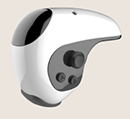
\includegraphics[width=\textwidth]{tactai}
	\captionsource{Urządzenie Tactai}{\url{https://www.tactai.com/company}\\}
	\label{fig:tactai}
	\end{subfigure}
	\hspace{0.5cm}
	\begin{subfigure}[b]{0.4\textwidth}
	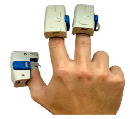
\includegraphics[width=\textwidth]{touchVr}
	\captionsource{Urządzenie TouchVr}{\url{https://www.gotouchvr.com/copy-of-technology-devices-1}}
	\label{fig:touchVr}
	\end{subfigure}
\caption{Urządzenia nasadowe.}
\label{fig:tactails}
\end{figure}

	\subsection{Egzoszkielety}
	\label{subsec:egzo}	
	Ostatnim rodzajem kontrolerów które bazują na ruchu dłoni i zarazem tych które podejmują niejako największe wyzwanie są egzoszkielety. Rękawica typu egzoszkielet, jak sama nazwa wskazuje, jest to rodzaj rękawicy posiadający swojego rodzaju szkielet zewnętrzny. Szkielet ten przymocowany wokół rąk użytkownika służy jako dodatkowa blokada dłoni, dzięki czemu użytkownik świata wirtualnego otrzymuje te same odczucia oporu wynikające z przedmiotów jak w świecie rzeczywistym. Gdy w świecie wirtualnym użytkownik takiego szkieletu ściska kamień, jego dłoń jest blokowana w odpowiednich miejscach, w zależności od danych uzyskanych ze świata wirtualnego który definiuje to jaką pozycję ręka użytkownika może maksymalnie przyjąć. Jest to rodzaj kontrolera nasadowego który pozwala poczuć świat wirtualny jednak nie w dosłownym tego znaczeniu. Uzyskane w ten sposób uczucia nie imitują dotyku przedmiotu a jedynie symulują opór jaki te przedmioty wytwarzają. Ludzki mózg jednak zawsze stara znaleźć się wyjaśnienie dla danego zjawiska, w związku z tym samoistnie łączy bodźce wzrokowe z blokadą motoryczną ręki, nadając tym samym generowanym komputerowo przedmiotom wyższy realizm. Istnieje wiele firm zajmujących się tego typu projektami jednak w tym rozdziale zostanie opisane tylko kilka których w sposób szczególny wyróżniają się na tle konkurencji.
	 Projekt taki stworzyła chińska firma Dexta Robotics, która wystartowała z kampanią finansowania społecznego w 2014 roku, jednak zbiórka pieniędzy zakończyła się niepowodzeniem. Była to jedna z pierwszych  spopularyzowanych rękawic egzoszkieletów, która pomimo porażki w zbiórce pieniędzy przetrwała i firma dokończyła projekt na własną rękę w 2016 roku. Egzoszkielet ten pozwala zatrzymać rękę gdy trafi na odpowiedni obiekt a także stopniowo aplikować opór gdy jest ściskany obiekt który ten opór zmienia w zależności od poziomu nacisku. Minusem tego rozwiązania jest opór który zostaje nakładany jedynie na czubki palców, co sprawia że traci się w pewnym stopniu realizm interakcji. Sam wygląd rękawicy jest natomiast bardzo futurystyczny - rękawica przedstawiona jest na rysunku~\ref{fig:dexmo}~\cite{dexta}.
	 \begin{figure}[h]
	 \centering
	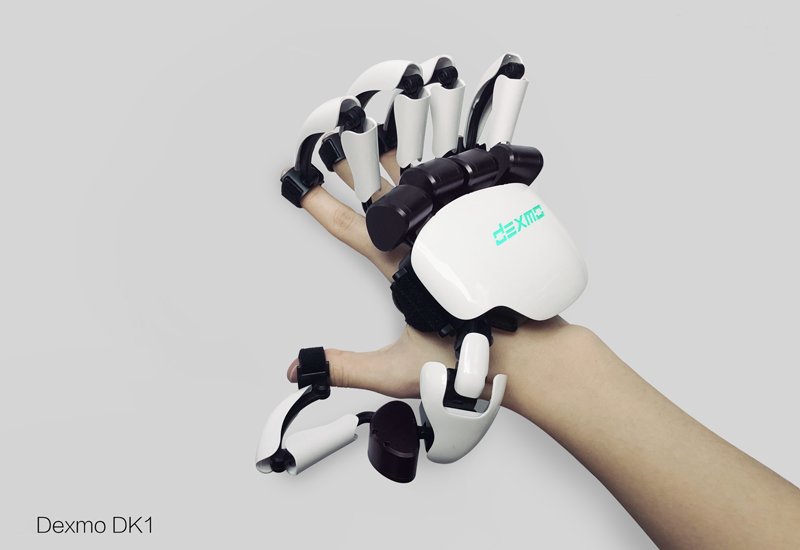
\includegraphics[width=0.7\textwidth]{dexmo}
	\captionsource{Egzoszkielet firmy Dexta Robotics}{\url{https://www.dextarobotics.com/en-us/stories}}
	\label{fig:dexmo}
	\end{figure}	
		\begin{wrapfigure}{l}{0.5\textwidth}
\begin{center}
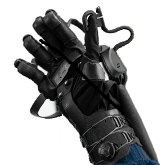
\includegraphics[width=0.46\textwidth]{haptx}
\captionsource{Egzoszkielet firmy HaptX}{\url{https://www.purepc.pl/haptx-glove-pozwoli-na-rejestrowanie-bodzcow-czuciowych-w-vr}}
\label{fig:haptx}
\end{center}
\end{wrapfigure}
	 Kolejnym projektem godnym uwagi jest rękawica HaptX, która pomimo dość dużych rozmiarów, niezbyt zgrabnego wyglądu oraz wagi około 2,5 kg dostarcza wyjątkowe funkcjonalności. Po pierwsze rękawica ta posiada 120 płytek wokół całej dłoni które imitują nacisk przedmiotów w świecie wirtualnym. Płytki te to małe kółka (około 2-3 mm) zgrupowane na płytce po kilka, kilkanaście sztuk w zależności od umiejscowienia na dłoni, w celu lepszej dystrybucji oraz możliwości zarządzania nimi. Rękawica jest na tyle dokładna że można poczuć pojedyncze odnóża chodzącego po dłoni pająka. Firma pracuje również na dodaniem właściwości termicznych do tych płytek co oprócz dotyku pozwoliłoby poczuć temperaturę przedmiotów. W drugiej generacji rękawicy można było poczuć ciepło oraz zimno dzięki zastosowaniu ciepłego i zimnego płynu którymi wyżej wymienione płytki się napełniają. Informację o położeniu naszej dłoni są wyliczane na podstawie dwóch źródeł. Jednym jest śledzenie optyczne naszej dłoni, drugim natomiast położenie naszych palców względem siebie wyliczane dzięki czujnikom magnetycznym które znajdują się na czubkach palców. Rękawica pokazana jest na rysunku~\ref{fig:haptx}~\cite{haptx}.
	 Cyber grasp to rozwiązanie które powstało w 2013 roku, gdy popularność VR znowu zaczęła wzrastać. Jest to egzoszkielet który w pełni kontroluje ruchy naszych palców u dłoni. Jest on nakładany na rękawice które zbiera dane o dłoni. Egzoszkielet jest dość duży i mało przyjazny dla oka, nadrabia to jednak funkcjonalnością oraz solidnym wykonaniem. Zapewnia on pełną swobodę ruchu, do 12 N nacisku oraz możliwość zaprogramowania osobno każdego siłownika oddziałującego na poszczególny palec. Sama rękawica zapewnia osiemnaście sensorów - dwa sensory zgięcia na każdym palcu, cztery sensory odwodzenia pomiędzy palcami, sensor mierzący ruch kciuka, kąt dłoni, a także wygięcie oraz odwodzenie nadgarstka. Istnieje również wersja z czterema dodatkowymi sensorami która zapewnia po jednym dodatkowym sensorze na wszystkie palce poza kciukiem. Oprogramowanie rękawicy wspiera imitację takich odczuć jak pulsowania oraz wibracji dla lepszych doznań ze świata wirtualnego~\cite{cyber}. Ostatnim urządzeniem opisanym w tej sekcji jest rękawica firmy Cynteract. Jest to niemiecka grupa studentów produkująca kontroler w postaci przypominającej egzoszkielet. Nie jest to szkielet w dosłownym tego słowa znaczeniu, a raczej rękawica z zaimplementowanym mechanizmem na wierzchu dłoni, który oddziałuję z małą siłą na palce dłoni. Małe silniki kontrolują napięcie sznurków które wędrują wzdłuż palców aż do samych czubków zapewniając odpowiedni opór. Nie jest to mechanizm który ma na celu powstrzymanie zgięcia dłoni a jedynie stawianie regulowanego oporu. Głównym celem tego produktu jest dotarcie do osób które mają problemy z kontrolowaniem dłoni, dzięki czemu przy użyciu tej techniki mogą dokonywać rehabilitacji w bardziej przyjemny sposób poprzez granie w specjalnie zaprogramowane gry które jednocześnie zbierają dane na temat progresu pacjenta.Rękawica jest uniwersalna dzięki czemu technologia użyta na wierzchniej części może być wymieniania pomiędzy różnymi wersjami tego produktu - oprogramowanie stojąca za działaniem tego mechanizmu jak i rękawicy samej w sobie kryje się w pojemniku umocowanym na nadgarstku. Jest to produkt który nastawiony jest konkretnie na branżę medyczną a jego rozwój wspiera wiele placówek medycznych na terenie Niemiec które już z tego rozwiązania korzystają~\cite{act}. Oprócz wspomnianych projektów istnieje wiele innych rozwiązań implementujących własne rozwiązania problemów kontroli ciała użytkownika. Coraz więcej firm stara się aby ich produktu oprócz wysyłania informacji ze świata rzeczywistego do świata wirtualnego, w celu jak najlepszego odwzorowania użytkownika w tym uniwersum, zapewniało również połączenie w drugą stronę, tak aby ich produkty reagowały na interakcję świata wirtualnego w świecie rzeczywistym, pogłębiając tym samym imersje użytkownika. W tej pracy poruszono jedynie tematykę egzoszkieletów bazujących na kontroli palców, istnieją jednak inne rozwiązania które wykorzystują bardziej skomplikowane systemy, również łączące w sobie wiele rozwiązań z rożnych firm, pozwalające wpływać na poruszanie się ciała użytkownika. W skład tych systemów zazwyczaj wchodzą również rękawice, jednak celem tych produktów nie jest imitacja dotyku poprzez ograniczenie ruchu na której się skupiono w tej sekcji. 
\chapter{Zastosowania w biznesie}
\label{ch:biznes}
 Technologia wirtualnej rzeczywistości zajmuje umysł rozmyślaniem nad nieskończonymi możliwościami inwestorom, podmiotom biznesowym oraz twórcom od  dawna. Pomimo swoich początków w branży rozrywkowej coraz więcej osób dostrzega potencjał tej technologii w zastosowaniu biznesowym. Znajomość technologiczna pracowników pozwala na wdrożenie rozwiązań VR bez większych problemów a przypadki biznesowe dla których zostają wprowadzone rozwiązania z tej dziedziny często pozwalają na redukcje kosztów oraz czasu, w szczególności jeżeli porównywane jest to do odtworzenia danego środowiska w przestrzeni rzeczywistej, o ile to jest w ogóle możliwe. W wielu dziedzinach takich jak medycyna, motoryzacja, architektura czy lotnictwo coraz częściej liderzy decydują się na inwestycje oraz współpracę z firmami z obszarów XR, a dzięki przetartym szlakom, także kolejne branże coraz chętniej przyglądają się możliwościom zastosowania narzędzi pozwalających na tworzenie środowisk wirtualnych. Prognozy rynku przez takie firmy i agencje jak \textit{The Farm 51}, \textit{Tractica}, \textit{CCS Insight} czy \textit{SuperData} pokazują że wartość aplikacji oraz akcesoriów związanych z sektorem VR będzie ciągle rosnąć i stawać się coraz bardziej powszechna wśród użytkowników domowych, co sprawia że potencjał inwestycji dla wielu firm również wzrośnie, nawet jeżeli nie zdecydowały się one na wdrożenie rozwiązań technologicznych na chwilę obecną~\cite{raportVR}. Dzięki prężnemu rozwojowi technologii oraz coraz większemu zaufaniu tej technologii, miało szansę powstać wiele firm które nie tylko zajmuje się produkcją fizycznych komponentów o których wspomniano w rozdziale~\ref{ch:prezentacja}, ale także firmy które zajęły się wytwarzaniem oprogramowania oraz współpracy z klientami.
 \begin{figure}[h]
\centering
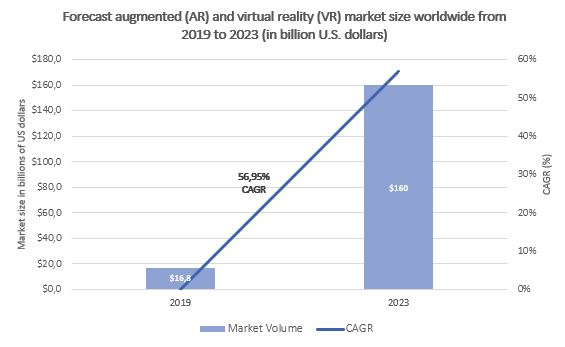
\includegraphics[width=\textwidth]{market}
\captionsource{Przewidywania wartości rynku AR i VR pomiędzy 2019 a 2023 rokiem}{\url{https://blog.camelot-group.com/2020/01/ar-vr-mr-science-fiction-or-science-fact/}}
\label{fig:market}
\end{figure}
  Firmy te zajmują się wytwarzaniem oprogramowania z którego mogą korzystać inne osoby w celu budowania własnych rozwiązań, firmy współpracujące z klientami i zajmujące się wdrażaniem ich pomysłów w życie, co często można zaobserwować w segmencie rozrywkowym a także jednostki zajmujące się produkcją oprogramowania z wyszczególnieniem danych sekcji przemysłowych, do których potrzebna jest bardziej szczegółowa wiedza i zazwyczaj firmy takie zajmują się tylko jednym rodzajem dostarczanych rozwiązań takich jak usprawnianie linii przemysłowych, usprawnianie napraw i rutynowych kontroli czy też tworzenie symulatorów w celu wydajniejszego szkolenia pracowników. Aktualnie do najlepszych firm na rynku, które oferują swoje rozwiązania klientom należą takie firmy jak \textit{VironIT}, \textit{Next/Now}, \textit{HQSoftware} czy też \textit{Notion Theory}. Segment ten jest wciąż powiększający się, co daje szanse wielu przedsiębiorcom na rozpoczęcie własnej działalności w dostarczaniu rozwiązań XR w wielu dziedzinach biznesowych. Wartość rynku  wirtualnej oraz rozszerzonej rzeczywistości w  roku 2019 wyniosła 16,8 miliarda dolarów i od tamtej pory wciąż rośnie. Prognoza rynku VR/AR na najbliższe lata jest pokazana na rysunku~\ref{fig:market}. Rysunek ten pokazuję również CAGR (z ang. Compound Annual Growth Rate) czyli skumulowany roczny wskaźnik wzrostu, rysując prostą linię wzrostu na poziomie prawie 57\%. 
   \begin{figure}[h]
\centering
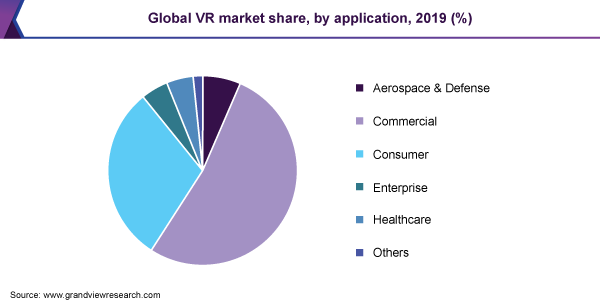
\includegraphics[width=\textwidth]{market_markets}
\captionsource{Światowy podział rynku VR pod względem wykorzystania aplikacji na rok 2019}{\url{https://www.grandviewresearch.com/industry-analysis/virtual-reality-vr-market/}}
\label{fig:market_m}
\end{figure}
 Poniżej przedstawiono kilka obszarów biznesowych w których rozwiązania XR funkcjonują często od wielu lat a ich rozwój i usprawnianie ciągle trwa. Do tych obszarów należą obszary takie jak lotnictwo, przemysł, medycyna oraz rozwiązania komercyjne~\cite{firmy}~\cite{vr4bus}. Obszary te zostały wybrane ze względu na popularność rozwiązań prezentowanych na rynku. Podział ten przedstawia rysunek~\ref{fig:market_m}.
\section{Lotnictwo i przemysł}
\label{sec:lotnictwo}
 Symulatory lotów były używane w szkoleniach wojskowych od wielu lat, ze względu na koszta które wynikały z używania prawdziwych samolotów jak i również potencjalnych zniszczeń który mogły powstać w trakcie szkolenia, a także bezpieczeństwa które symulator zapewniał. Dzięki temu popełnione błędy nie skutkowały utratą życia pilota. Równie ważnych aspektem jest fakt że podczas korzystania z symulatora można przetestować pilota w sytuacji awaryjnej, w której to należy podejmować szybkie decyzje a moment nie uwagi skutkuje rozbiciem maszyny. Dzięki temu w prawdziwej walce piloci są pewniejsi siebie oraz podejmują lepsze decyzje. Pierwsze symulatory powstały na początku XX wieku i były wykonane z drewna. Z biegiem czasem i rozwoju technologii pod koniec tego samego wieku zastąpiły je symulatory bazujące na mechanicznych częściach dzięki którym możliwy był ruch kokpitu, a obraz był wyświetlany na ekranach o dużej rozdzielczości. Koszty takiej maszyny mogły nawet przekraczać miliony dolarów. W związku z tym nastanie ery hełmów dla wirtualnej rzeczywistości przyniosło wiele rozwiązań które szybko zostały zastosowane. Dzięki użyciu gogli wyświetlających obraz, zwiększył się realizm or imersja symulacji, wizja pilota jest odwzorowana z uwzględnieniem ostrości widzenia, przeciążeń a także zapewniona jest wybiórcza wizja $360^o$, czyli pokazywany jest jedynie obszar widoczny w polu widzenia pilota, jednak może on dowolnie obserwować otoczenie wokół niego~\cite{del}. Kolejną instytucją w której wykorzystuje się technologie VR do szkolenia pracowników jest NASA. Wykorzystywanie nowoczesnych technologii w tej agencji kosmicznej nie jest nowością. W tym przypadku NASA zaprezentowało swój nowy symulator przeznaczony dla astronautów wyruszających na międzynarodową stację kosmiczną. W tym celu została wykorzystana technologia MR, dzięki której oprócz wirtualnych przedmiotów widzianych przez kosmonautę, były one również umiejscowione w tym samym miejscu w świecie rzeczywistym. Taki rodzaj symulacji zapewniał wyższy poziom realizmu przy zachowaniu niskich kosztów. System ten wspiera współpracę wielu użytkowników jednocześnie dzięki czemu zadania które są wykonywana w symulacji mogą również uwzględniać współpracę pomiędzy członkami załogi~\cite{nasa1}. Innym rodzajem symulacji, bazującym na treningu personelu są szkolenia personelu lotniczego. Nie dotyczy to jednak jedynie pilotów maszyn. Symulację dla personelu podczas pożaru w samolocie stworzyła firma EpicVR, która poprzez praktykę pokazała że pomimo dokładnych szkoleń i procedur, personel pokładowy wciąż popełnia błędy. Praktyka w symulatorze, dzięki zastosowaniu gogli do wirtualnej rzeczywistości sprawiła że już po kilku treningach, niektóre osoby wykonywały bezbłędnie procedury. Oczywiście praktyka takich procedur jest wykonywana nawet bez dostępu do nowoczesnej technologii, jednak w tym celu wymagana jest fizyczna wersja symulatora które nie są powszechnie dostępne~\cite{epicvr}. Są to jedynie przykładowe rozwiązania z tej dziedziny, z racji tego że wielkość fizycznych symulatorów pociąga za sobą duże koszta, wiele firm decyduje się na rozwiązania wirtualne. Innym sposobem stosowania symulacji jest symulacja linii produkcyjnej zastosowanej w Fordzie. Firma ta wprowadziła rozwiązania z dziedziny wirtualnej rzeczywistości zmniejszając ryzyko urazów o $70\%$, dla ponad 50 000 pracowników. Według danych podanych przez firmę, na dwa-trzy lata przed rozpoczęciem pracy nad nowym modelem zespół specjalistów analizuje w środowisku wirtualnym rozmieszczenie komponentów linii produkcyjnej tak aby zoptymalizować użycie siły pracowników aby nie doszło do przemęczenia, które mogłoby być przyczyną wypadku w fabryce. Aby osiągnąć najlepsze rezultaty podczas zbierania danych i zapewnić wymaganą jakość, zespół ten przeprowadza ponad 900 wirtualnych zadań zanim zostanie one fizycznie zbudowana, a oprócz podstawowych komponentów wykorzystują również technologie takie jak śledzenie ruchów całego ciała a także druk 3D~\cite{ford1}.
 
 Łatwo jest zauważyć jak duży wpływ rękawice wirtualnej rzeczywistości mają wpływ w tym obszarze rynku. Jeżeli firma chce symulować świat rzeczywisty w celu jak najlepszego szkolenia swoich pracowników, zależy jej aby były do tego wykorzystywane realne narzędzia. Będąc pilotem samolotu czy pracując fizycznie wykorzystujemy do tego nasze dłonie, w związku z tym podczas wykorzystania ich w trakcie treningu, ludzie również nabierają pamięci mięśniowej co pozwala podnieść poziom szkolenia a także rezultatów które dzięki niemu można osiągnąć. Między innymi ze względu na te powody, agencje takie jak NASA inwestują w technologię rękawic kontrolerów, sprawiając że powszechne rozwiązania symulatorów które będą wykorzystywane między innymi lotnictwie stają się coraz powszechniejsze~\cite{manus}. 
 
 \section{Architektura i wizualizacje}
\label{sec:architektura}
	Architekci jak mało która grupa deweloperów potrafią wykorzystać możliwości oferowane przez świat wirtualny. Od dawna grafika 3D jest powszechnie wykorzystywana w celu wizualizacji projektów, dzięki czemu klient bądź członkowie zespołu mają wgląd w to jak projekt będzie wyglądać po ukończeniu - wizja ta jest motorem napędowym całego projektu. DigitalVr postanowiło więc wykorzystać ten fakt i przenieść prezentację modeli na nowy poziom. Dzięki wykorzystaniu gogli VR, odbiorca jest w stanie przenieść się do ukończonego budynku zaprojektowanego w świecie wirtualnym, przejść się po nim, zmienić kolory ścian, obejrzeć je za dnia jak i nocy bądź poprzestawiać meble w pomieszczeniu. Jak twierdzą twórcy jest to swoiste przekazanie kluczy do drzwi wejściowych na lata przed powstaniem projektu w rzeczywistości. Twórcy wierzą że dzięki możliwością jakie zapewnia ich produkt, pewnego dnia ich rozwiązanie stanie się powszechnie używane. Obecnie rozwiązania takie nie tylko są oferowane przy użyciu gogli VR ale również aplikacji na smart-fony, które przy użyciu kamery telefonu pozwalają dopasowywać meble w pomieszczeniach domu bez opuszczania jego progu~\cite{arch}. Nie tylko architekci jednak wykorzystują wizualizację pomieszczeń w celu  przyciągnięcia klientów. Hotel Mariott International zamontował w niektórych swoich hotelach angielskie, czerwone budki telefoniczne w których można było skorzystać z zestawu Oculus Rift dzięki któremu klienci mogli przenieść się w wirtualną podróż do Londynu i na Hawaje~\cite{hotel2}. Współcześnie hotele takie jak Atlantis w Dubaju, Grand Oasis czy nawet powszechnie spotykany Holiday Inn oferują swoim klientom wirtualne wycieczki po hotelu zanim jeszcze zdecydują się na pobyt w ich posiadłości. Dzięki temu klienci wiedzą dokładnie na jakie atrakcje i standard mogą liczyć przy wyborze pokoju i lokacji~\cite{hotel1}. Wizualizacje przy wykorzystaniu XR nie służą jedynie przyciągnięciu klientów. Powszechnie stosuje się rozwiązania MR, AR oraz VR w celu optymalizacji pracy oraz redukcji błędów popełnianych przez pracowników.  Redukcja błędów jest szczególnie ważna w firmie Lockheed Martin, która wykorzystuje rozwiązania rozszerzonej rzeczywistości w celu budowania swoich samolotów wojskowych F-35. Wdrożenie tej technologii pozwoliło na zastąpienie grupy  wyszkolonych techników z latami doświadczenia, aplikacją która pokazuje pracowników jakie części muszę znaleźć się w danym elemencie. Brak zapamiętywania schematów a także aplikacja czuwająca nad pracą podczas składania poszczególnych elementów pozwoliła firmie usprawnić produkcję o $30\%$ a także uzyskać dokładność produkcyjną nawet do $96\%$. Podobną technikę wykorzystuje firma Boeing, która podczas montażu swoich samolotów wykorzystuje interaktywne instrukcje dzięki czemu w dowolnym momencie w łatwy sposób pracownicy mogą sprawdzić brakujące informacje. Jest to również zdecydowanie wygodniejsza forma niż manualne przeglądanie papierowych szkiców. Unikanie instrukcji papierowych jest stosowane nie tylko w przypadku  konstrukcji produktów lecz także podczas ich naprawy. Przykładem takiego zastosowania jest Panasonic Heating and Cooling Solutions - jest to dział ogrzewania i chłodzenia należący do firmy Pansonic. Dział ten wdrożył nowoczesne rozwiązanie dla swoich techników, pozwalając im przy wykorzystaniu  mieszanej rzeczywistości na konsultacje techników z centralą w celu rozwiązywania skomplikowanych problemów. Centrala po otrzymaniu obrazu jest w stanie na ekranie technika zaprezentować rozwiązanie danego problemu, znacznie skracając czas naprawy oraz redukując możliwość popełnienia błędów~\cite{pana}. Firma Ford natomiast oprócz zastosowania nowoczesnych technologii w swoich autach, stosuje ją również na etapie produkcji, i to nie tylko na linii produkcyjnej tak jak opisano to w sekcji~\ref{sec:lotnictwo}. Kolejnym przykładem nowoczesnego wykorzystania jest etap projektowania nowych aut. w tym celu projektancie mogą korzystać z gogli VR w celu wizualizacji swoich produktów w rzeczywistej skali jeszcze zanim zostaną one wyprodukowane, co pozwala na lepsze dopracowanie szczegółów każdego z aut~\cite{wiz1}. Firma Ford nie jest wyjątkiem w branży - rozwiązania XR oraz produkty rękawic kontrolerów stosowane są również w innych koncernach motoryzacyjnych takich jak BMW, Audi czy Toyota~\cite{manus}. Ostatnim rodzajem wizualizacji która zostanie opisana w tej sekcji jest klejne rozwiązanie stworzone przez agencję kosmiczną NASA. Tom Grubb który pracował nad tym narzędziem zauważył że badanie przestrzeni kosmicznej w szczególności związanej z liczbami dotyczącymi gwiazd w galaktyce, odbywało się poprzez używanie przestarzałych narzędzi opartych na pracy wielu baz danych. W związku z tym stworzył model w świecie wirtualnym który pozwalał na modelowanie tych danych w przystępnej dla ludzi formie czego rezultatem było osiągnięcie potwierdzenia wniosków z którymi do tej pory środowisko astronomów się nie zgadzało~\cite{nasa2}.
	
	 W tej sekcji przedstawiono kilka kolejnych rozwiązań dostępnych w firmach i agencjach które już teraz wykorzystują idealny kontroler - ludzką dłoń a także sposób stosowania nowych technologii w celu optymalizacji pracy a także przyciągnięcia nowych klientów. Jak widać w zależności od sektora a nawet działu,wizualizacje są wykorzystywane do najróżniejszych celów pozwalając na coraz to wydajniejszą pracę i lepsze efekty.
	
\section{Medycyna}
\label{sec:medycyna}
 Jednym z zastosowań obecnie używanych jest wspomniany już produkt Cynteract pomagający w fizjoterapii dłoni poprzez stawianie oporu a także interaktywny świat pozwalający zamienić trening w zabawę. Fizjoterapie nie jest jedynym obszarem w którym wykorzystuję się świat wirtualny. Jednym z bardzo imponujących zastosowań jest produkt o nazwie Snow World (z ang. Śnieżny świat), stworzony przez uniwersytet w Waszyngtonie. Produkt ten został stworzony aby pomagać pacjentom szpitala którzy doznali poważnych poparzeń ciała. Poprzez zastosowanie gogli VR zostają przeniesieni do śnieżnego świata w którym poprzez wizualizacje śniegu, bałwanów, pingwinów oraz innych typowych dla zimnego klimatu zwierząt i wydarzeń, pacjenci  mogą doświadczyć uczucia chłodu który jest generowany jedynie w naszej wyobraźni, jednak jak pokazują badania - mają bardzo realny efekt. Standardową procedurą jest podanie opioidów takich jak morfina, która redukuje ból w trakcie gojenia ran, jednak podczas oczyszczania ran czy zmian opatrunków skóra pacjentów poddawana jest dodatkowemu podrażnieniu co u niektórych pacjentów powoduje poważny ból pomimo zastosowania środków znieczulających, ponieważ pacjenci potrafią ponownie przeżywać doświadczenie poparzenia ich ciała. System wirtualnej rzeczywistości został zastosowany w celu dodatkowej redukcji bólu podczas tych bolesnych zabiegów poprzez przekierowanie skupienia pacjenta z bólu który przeżywa do wirtualnego środowiska. Zabieg przeprowadzono podczas  gdy pacjent grał w gry wideo na konsoli a także podczas przebywania w świecie VR. Rezultaty pokazały że samo przeniesienie skupienia na grę nie jest wystarczające - zastosowanie wirtualnego świata zmniejszyło odczucia bólu przez pacjenta o połowę~\cite{snow}. Tak jak w przypadku lotnictwa, również lekarze muszą trenować aby szczegółowo poznać procedury podczas wykonywania operacji. W tym obszarze wirtualne środowisko również przychodzi z pomocą. Oprócz pokazywania dobrze znanych zabiegów, w środowisku wirtualnym lekarze mogą ćwiczyć skomplikowane zabiegi, tak aby w trakcie prawdziwego zabiegu osiągnąć jak najlepsze rezultaty, tym samym ratując często ludzie życie. Symulacje zabiegów należą do grupy dość typowego wykorzystania wirtualnego świata, ponieważ praktycznie w każdym zawodzie można użyć tej technologii do polepszania umiejętności pracowników. Jednak w przypadku lekarzy, zastosowanie zaawansowanych i dokładnych rękawic sprawia że osoba ćwicząca dany zabieg nabiera pamięci mięśniowej a także uczy się obsługiwać dokładnie jak w rzeczywistości narzędzia które są wykorzystywane, często przy nietypowych zabiegach. Inną metodą wykorzystania XR jest tworzenie rozwiązań pomagających leczyć zespół stresu pourazowego poprzez stopniową ekspozycję pacjenta do bodźców i zastąpienie naturalnej reakcji pozytywnymi bodźcami. W podobny sposób tego rodzaju wizualizacje pozwalają pozbyć się różnego rodzaju lęków bądź nawet fobii takich jak lęk przed lataniem, wysokością, małymi pomieszczeniami czy wystąpieniami publicznymi. Wymienione zastosowania dobrze sprawdzają się w specjalistycznych placówkach, jednak istnieją również rozwiązania które dbają o ogólnie pojęte zdrowie człowieka poprzez naukę lepszego zarządzania stresem, relaksacji czy poprzez kurs medytacji - tego rodzaju rozwiązania mogą być wykorzystywane przez każdego z dostępem do gogli, sprawiając że ich użytek może być wyniesiony poza strefę rozrywkową~\cite{medycyna}.

\section{Rozrywka}
\label{sec:gry}
	Ostatnim działem opisanym w tej pracy jest jednocześnie strefa biznesu która rozpoczęła rozwój rynku wirtualnej rzeczywistości, dając jednocześnie początek innym technologiom a także pozwalając twórcą na wyobrażanie sobie coraz to nowych zastosowań w wielu dziedzinach biznesowych. Branża rozrywkowa poczynając od pierwszej maszyny Sensoramy aż do nowoczesnych gogli, napędza rynek konsumencki, sprawiając że technologia ta rośnie w popularności a także ludzie coraz częściej wiedzą jak z niej korzystać dzięki czemu łatwiej jest adoptowana w firmach. Mówiąc o rozrywce VR, najczęstszym skojarzeniem są gry komputerowe, które różnią się od bycia dokładnym odzwierciedleniem rzeczywistości do kompletnych abstrakcji. Oczywiście wszystkie opisane do tej pory zastosowania w biznesie, niejako mogą służyć jako przykłady dla gier. W ten sposób zostały stworzone symulatory lotów, które służą jedynie rozrywce, lecz często mogą być dobrym odwzorowaniem prawdziwego samolotu. W kontekście gier często użytkownik może sterować maszynami nie tylko powietrznymi ale także rożnego rodzaju pojazdami naziemnymi oraz wodnymi. Większość gier komputerowych które na chwilę obecną są wyświetlane na ekranie komputera, może zostać przeniesionych do VR, często z lepszymi doświadczeniami płynącymi z gry. Do najbardziej popularnych gier należą gry typu FPS (z ang. First Person Shooter), czyli gry polegające na strzelaniu i pokonywaniu przeciwników w których wcielamy się w postać i widzimy niejako jej oczami. Gracze mogą doświadczyć realnych wrażeń poprzez znalezienie się w środku pola bitwy, widoku i dzwięku eksplozji a także strzałów wokół nich. Do najpoważniejszych problemów tego typu gier należy możliwość poruszania się w świecie wirtualnym, tak aby był zachowany jak największy realizm. Kolejną pozycją która zajmuję dużą część rynku gier VR, są gry typu horror. Poprzez zastosowanie wizji $360^o$, wysokiej jakości grafiki, nastrojowego dźwięku oraz gwałtownych interakcji, gry te przenoszą użytkownika na wyższy poziom doznań, a w końcu to jest to czego fani tego typu gier oczekują. W przeciwieństwie do wymienionych do tej pory gatunków, wspomniane wcześniej symulatory nie cierpią z powodu problemu poruszania się, co sprawia że inercja użytkownika jest większa. Istnieją również gry strategiczne a także hazardowe które nie wymagają od użytkownika poruszania się, jednocześnie dostarczając lepszych doznań poprzez symulacje przebywania na polu bitwy na którym mamy widok "od środka" bądź też gdy użytkownik znajduję się w wirtualnym kasynie podczas gry w pokera~\cite{gry1}. Doświadczając rozrywki wirtualnego świata, należy wspomnieć o grze która przyczyniła się do rozgłosu technologii VR oraz jej popularyzacji jak żadna inna - Beat Saber to gra w której kontrolery zamieniają się w miecze w dwóch kolorach, którymi następnie należy niszczyć nadciągające w stronę użytkownika bloki. Bloki te mają kolory odpowiadające mieczom, i jedynie ten sam kolor miecza może je zniszczyć. Z pozoru bardzo prosta gra, jednak przyciągnęła ona wielu fanów a w szczególności pokazała przeciętnym graczom że może być tak ekscytująca jak gry 2D. Beat Saber sprzedała się w ilości ponad 100 000 egzemplarzy w przeciągu pierwszego miesiąca i została siódmą co do najlepiej ocenianych gier na platformie dla graczy Steam, pośród gier 2D jak i VR~\cite{gry2}. 
Oprócz zwykłych gier które służą czystej rozrywce, istnieje również zastosowanie gier w celach edukacyjnych. Gry takie wykorzystują stworzone środowisko w celu wizualizacji przedstawianego tematu w sposób bardziej intuicyjny niż samo opisywanie słowami, co wspomaga naukę u dzieci a nawet budzi większe zainteresowanie tematem. Do takich aplikacji należą na przykład aplikacje takie jak  Titans of Space, które prezentują układ słoneczny - do tej pory jedyną możliwością była prezentacja modeli które są wykonana w dużym pomniejszeniu. Innym przykładem jest aplikacja Anatomyou, która pozwala na podróż w głąb ludzkiego ciała. Rozwiązanie to sprawdza się w przypadku nauki biologii i anatomii. Istnieje wiele produktów które są przeznaczone do edukacji i szkoleń a rynek związany z grami wciąż rośnie~\cite{gry3}. Poniżej, na rysunku~\ref{fig:market_gry} pokazany jest podział rynku gier ze względu na wymagane komponenty. Rynek jest warty miliardy oraz wciąż rośnie co otwiera wiele możliwości zarówno dla twórców gier służących rozrywce jak i edukacji. Stwarza to możliwości zarówno dla nowych studiów produkcyjnych jak i dla biznesów zajmujących się wcielaniem w życie pomysłów dostarczonych przez inne osoby~\cite{gry1}.
   \begin{figure}[h]
\centering
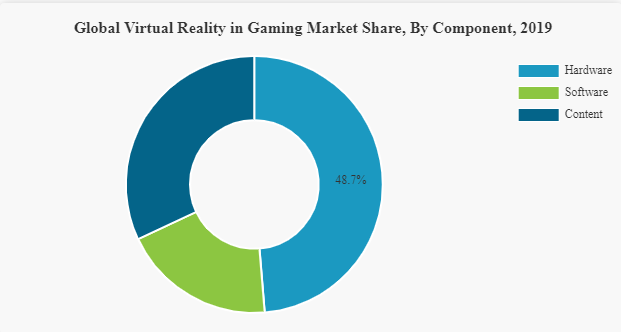
\includegraphics[width=\textwidth]{market_gry}
\captionsource{Światowy podział rynku gier VR pod względem komponentów na rok 2019}{\url{https://www.fortunebusinessinsights.com/industry-reports/virtual-reality-gaming-market-100271}}
\label{fig:market_gry}
\end{figure}
\chapter{Projekt rękawicy}
\label{ch:projekt}
Istotą poniższego rozdziału jest pokazanie użytych w projekcie podzespołów i technologii oraz lepsze zrozumienie powodów dla których to właśnie te produkty zostały wybrane. Po zapoznaniu się z motywem, zostanie szczegółowo opisana specyfikacja tych produktów a także sposób ich poskładania w spójną całość, co sprawiło pewne problemy względem oryginalnego szkicu - próby oraz efekty rozwiązywania tych problemów również zostaną opisane w tym rozdziale. Po nakreśleniu podstawowych założeń projektu zostanie zaprezentowana finałowa wersja, a także szczegółowo zostanie omówiony kod rękawicy-kontrolera, który jest obsługiwany przez mikrokontroler i stanowi najważniejszą część tego projektu.
\improvement{proof read}
\improvement{Opis: BLE, Rotacja, przesunięcie i animacja, przy opisywanych sensorach}


\section{Przegląd podzespołów użytych w projekcie}
\label{sec:przeglad}
Jak dowiedzieliśmy się z rozdziału \ref{ch:komponenty} dotyczącego podstawowych komponentów rękawic, kluczowym dla powodzenia projektu jest ustalenie następujących pozycji: 
\begin{itemize}
\item orientacji dłoni względem punktu początkowego
\item położenia względem punktu początkowego
\item moment i stopień zgięcia palców 
\end{itemize}
 W tym celu należy zebrać informacje z czujników, a następnie wszystkie te informacje należy przesłać do pożądanego urządzenia. Elementem które pozwala to osiągnąć w tym projekcie jest mikrokontroler Arduino nano 33 BLE, który odpowiada za dostarczenie informacji z żyroskopu, akcelerometru a także czujników wygięcia. Zasady działania pierwszych dwóch zostały opisane z podrozdziale~\ref{subsec:sensory}. Natomiast w poniższych podrozdziałach zostanie opisane rozwiązanie zastosowane do odczytu położenia palców, zasada działania przy wykorzystaniu rezystorów oraz sposób połączenia wszystkich wspomnianych elementów w jeden finałowy kontroler.
	
	
	\subsection{Mikrokontroler}
	\label{subsec:arduino}
	Jak przed chwilą wspomniano, w projekcie wykorzystywana jest płytka od Arduino, która nosi nazwę Nano 33 BLE. Jest to małych rozmiarów płytka o  wymiarach 45 x 18 mm, pozwalająca na wysoką wydajność przy jednoczesnym małym poborze prądu, co zapewnia użyty mikrokontroler nRF52480 o taktowaniu 64 MHz. Do dyspozycji mamy również pamięć RAM o pojemności 256 kB oraz pamięć Flash o pojemności 1 MB. IMU które zostało zamontowane na płytce to LSM9DS1, które obsługuję akcelerometr, żyroskop oraz magnetometr w trzech osiach. Więcej infomracji na temat IMU jest przedstawione w części~\ref{sec:oprogramowanie}. Warto na wstępie zauważyć że Nano 33 BLE pracuje domyślnie wyłącznie z napięciem 3,3 V, w związku z czym nie należy podłączać bezpośrednio zasilania o większym napięciu. W celu podłączenia zasilania 5 V należy zlutować zworkę znajdującą się pomiędzy pinami RDT oraz A7 - temat ten nie zostaje jednak poruszony w tej pracy, ponieważ na potrzeby projektu używane jest zasilanie poprzez złącze micro USB które to również jest obsługiwane. Płytka ta posiada wiele użytecznych sensorów, jednak na potrzeby tej pracy została wybrana z powodu wbudowanej inercyjnej jednostki pomiarowej, dzięki czemu można było uprościć konstrukcję   oraz zmniejszyć ilość połączeń na rękawicy, wbudowanego modułu Bluetooth - a w tym przypadku modułu Bluetooth Low Energy obsługiwanego w standardzie 5.0, a to wszystko w przystępnej cenie co również było jednym z kryteriów przy tworzeniu tego projektu. Płytkę w momencie tworzenia tej pracy można kupić za 119 zł. Wartym uwagi jest fakt możliwości zakupu płytki bez wyprowadzonych złącz, co w przypadku opisywanego projektu pozwoli na zmniejszenie wymiarów oraz większą swobodę montażu~\cite{botland-arduino}.
\begin{figure}[h]
\centering
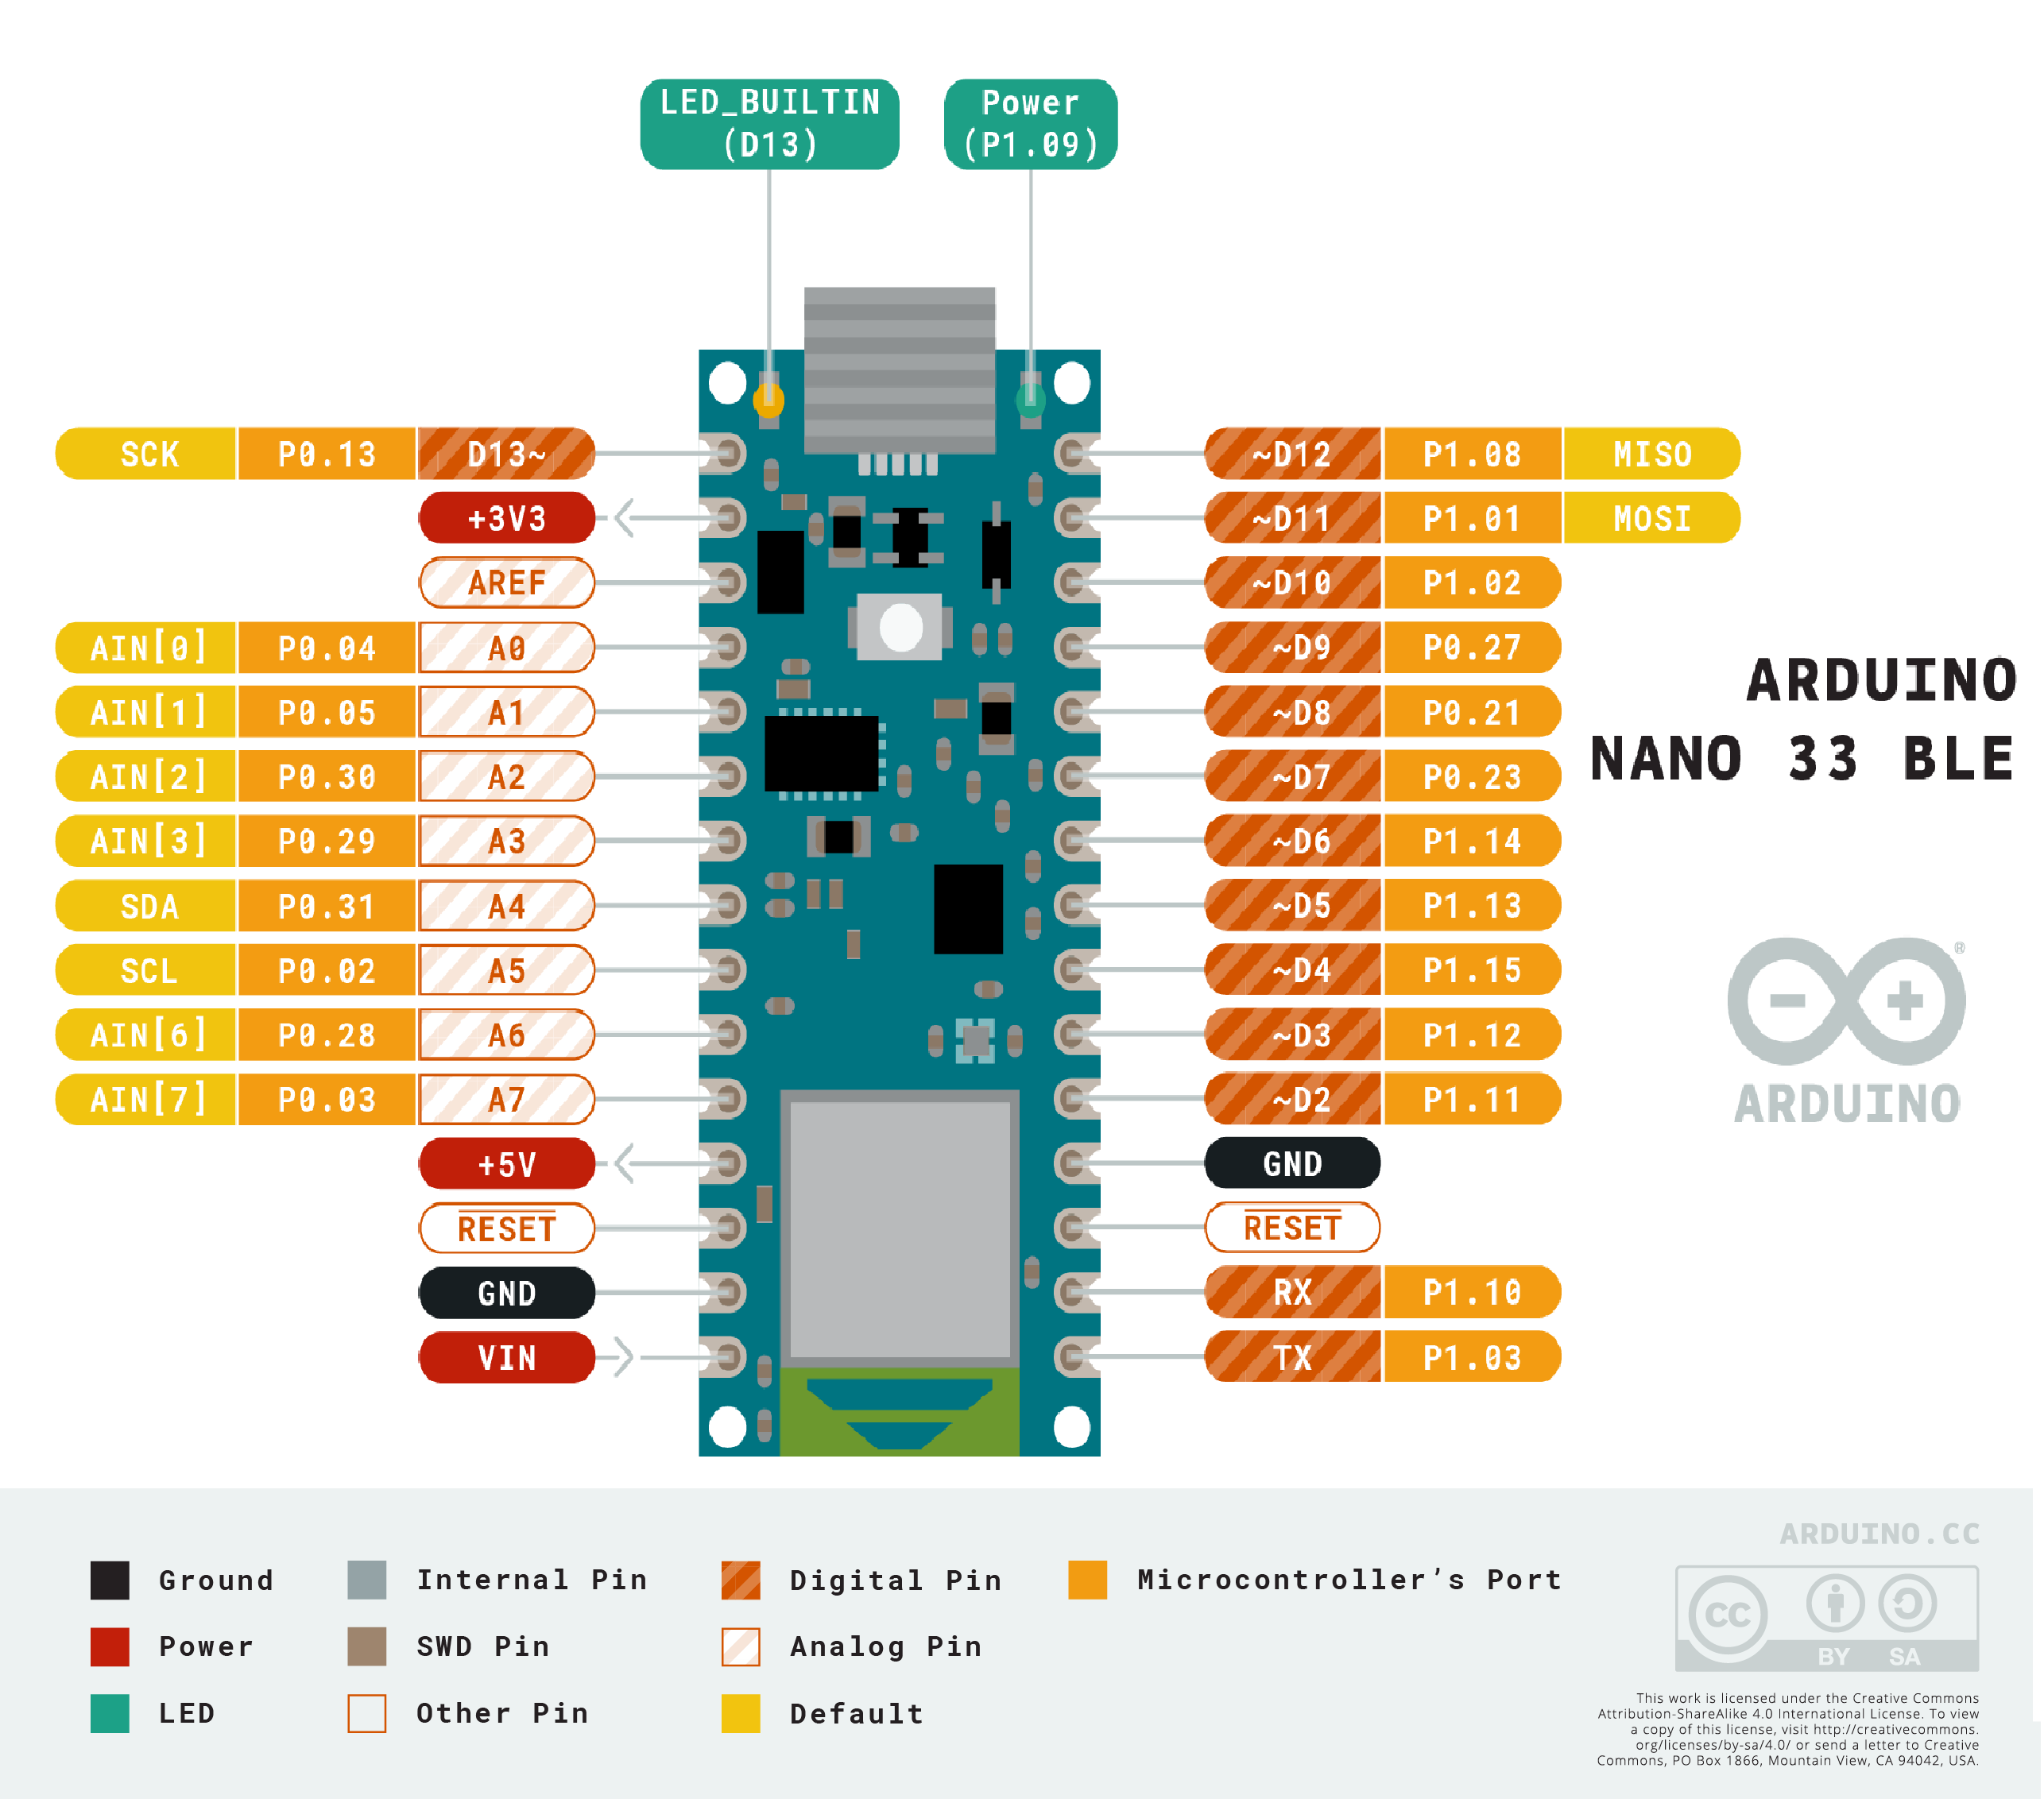
\includegraphics[scale=0.5]{arduino}
\captionsource{Opis wejść oraz wyjść Arduino Nano 33 BLE}{\url{https://content.arduino.cc/assets/Pinout-NANOble_latest.pdf}}
\label{fig:arduino}
\end{figure}
	
	Z najważniejszych elementów układu płytki należy wiedzieć że posiada ona dwie diody po dwóch stronach portu micro USB - zielona indykuje podłączone zasilanie, natomiast pomarańczowa zaczyna mrugać gdy jest przesyłany kod do mikrokontrolera. Oprócz tego do dyspozycji są dwa piny wyjściowe zasilające o napięciu 3,3 V oraz 5 V, jeden pin zasilający wejściowy, którego ograniczenia zostały wspomniane w poprzednim paragrafie, a także dwa piny uziemiające, po jednym z każdej strony płytki. Posiada ona piny zarówno analogowe jak i cyfrowe, jednak na potrzeby tego projektu zostały użyte jedynie piny analogowe, których do dyspozycji jest aż osiem umiejscowionych po jednej stronie, przy czym warto zwrócić uwagę że piny A4 oraz A5 używane są jako magistrala I2C w związku z czym zalecane jest nie stosowanie tych wejść analogowych. Szczegółowy opis wejść/wyjść płytki przedstawiony jest na grafice~\ref{fig:arduino}. W tym projekcie wykorzystano zasilanie poprzez złącze micro USB, wyjście o napięciu 3,3 V w celu uzyskania odczytów z czujników wygięcia na pinach analogowych A0, A1, A3, A6 oraz A7, o których zostanie więcej powiedziane w punkcie~\ref{sec:budowa}, a także uziemienie znajdujące się po tej samej stronie płytki.

	\subsection{Czujnik wygięcia}
	\label{subsec:wygiecie}	
	Kluczowym dla działania kontrolera jest możliwość określenia pozycji palców względem dłoni. Ma to wiele zastosowań zarówno wizualnych jak i praktycznych. Ważne jest aby odwzorować świat rzeczywisty tak dokładnie jak to możliwe - im lepsze odwzorowanie tym bardziej zmysły użytkownika zostaną oszukane, podwyższając komfort użytkowania technologii wirtualnej rzeczywistości. Za stroną praktyczną natomiast przemawia możliwość śledzenia palców w celu dokładnego ich użycia w stworzonym środowisku np. do ściskania i podnoszenia obiektów czy też korzystania z klawiatury wirtualnej. Jak wspomniano w rozdziale~\ref{ch:komponenty} dotyczącym komponentów komercyjnych rękawic - wśród znanych producentów na rynku, decyduję się na użycie wielu inercyjnych jednostek pomiarowych, na podstawie których są w stanie dokładnie określić położenia każdej części palca, bądź też nie aż tak popularne rozwiązanie, które wykorzystujące specjalistyczne sensory służące do pomiaru stopnia wygięcia czujnika względem pozycji prostej.
Czujnik ten po podłączeniu do prądu zwiększa swój opór wraz ze zwiększonym stopniem odchylenia. Oba te rozwiązania pomimo wysokiej dokładności pomiarów nie są rozwiązaniami tanimi. W związku z tym na potrzeby stworzenia taniego kontrolera, należało znaleźć rozwiązanie bardziej przystępna a jednocześnie pozwalające na osiągnięcie tego samego celu.
	
	Aby osiągnąć postawione założenia zostały skonstruowane czujniki wygięcia w domowych warunkach. Rozwiązanie to jest często używane do osiągnięcia pomiaru stopnia wygięcia bez konieczności wydawania ponad 100 zł na jeden czujnik~\cite{flex-sensor}. Jest ono stosunkowo proste w założeniach i wymaga jedynie dwóch kluczowych elementów. Tkaniny przewodzącej o specjalnych właściwościach oraz dwóch przewodników po obu stronach materiału. Z jednej strony zostanie podłączone napięcie z drugiej natomiast uziemienie. Ważnym jest aby połączenia te się ze sobą nie stykały w żadnym punkcie a jedynie zostały nałożone na siebie, z tkaniną ściśniętą pomiędzy nimi - dzięki temu mamy pewność że odczyty które otrzymamy będą prawidłowe. Pozostaje odpowiedzieć na pytanie jakiego rodzaju materiał należy wykorzystać. Na rynku znajdziemy wiele rodzajów materiałów które zmieniają swój opór w zależności od spełnienia takich kryteriów jak nacisk, temperatura, rozciągnięcie czy też właśnie zgięcie materiału. Pomimo próby uzyskania materiału który zmienia swój opór w zależności od rozciągnięcia, co pozwoliłoby na skonstruowanie części na palce rękawiczki z tego materiału, zapewniając dokładniejszy i bardziej estetyczny efekt końcowy, w momencie projektowania rękawicy był on jedynie możliwy do sprowadzenia ze stanów, co nie było najtańszym rozwiązaniem. W związku z tym zdecydowano się na użycie foli Velostat która jest czuła na nacisk or zginanie~\cite{velostat}. W roli przewodnika wybrano nić przewodzącą, która zapewniła potrzebną elastyczność oraz możliwość przymocowania poszczególnych elementów przy jednoczesnym zapewnieniu funkcjonalności. Elementy te zostały sklejone na kawałku taśmy samoprzylepnej oraz dodatkowo sklejone przy brzegu aby nić nie wyśliznęła się w trakcie korzystania z czujnika. Efekt końcowy jest widoczny na zdjęciu~\ref{fig:sensor}. W celu otrzymania pomiarów wszystkich palców zostało wykonanych pięć takich sensorów, o szerokości 15 mm; dwa o długości 8 cm, dwa o długości 10 cm a także jeden 11 cm, w celu jak najlepszego dopasowania względem miejsca na palce na zakupionej rękawicy do której sensory zostaną przymocowane, co można zobaczyć na zdjęciu~\ref{fig:glove}.
	
\begin{figure}[h]
\centering
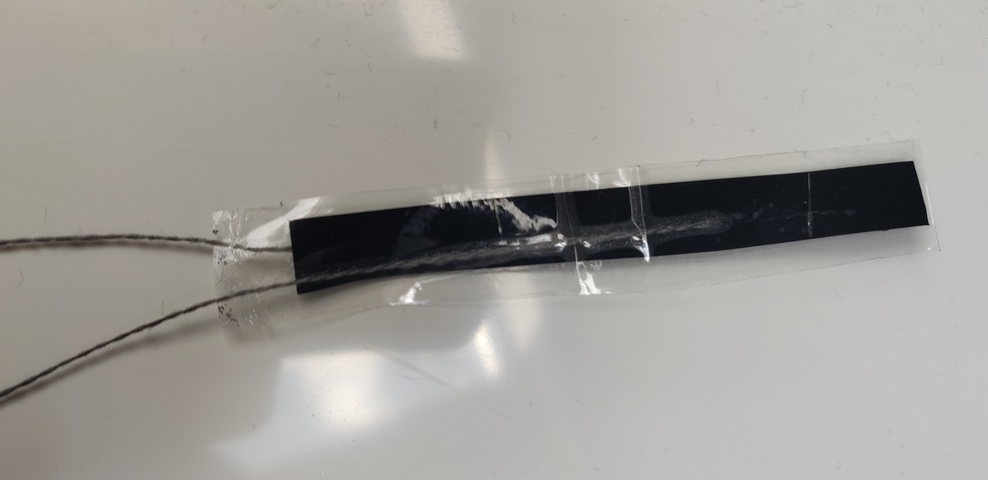
\includegraphics[scale=0.65,width=\textwidth]{flex-sensor}
\caption{Sensor wygięcia własnego wykonania}
\label{fig:sensor}
\end{figure}	

	\subsection{Rezystor}
	\label{subsec:rezystor}	
	Rezystor, potocznie zwany opornikiem, jest to prosty element elektroniczny, posiadający jedynie wyjścia z dwóch stron elementu łączącego. Element ten tworzy opór, powodując ograniczenie przepływającego przez niego prądu gdy jest włączony do obwodu szeregowo. Opór ten jest mierzony w omach. Istotną informacją jest fakt że nadmiar prądu jest zamieniany przez opornik na energie cieplną, a także brak zdefiniowanego kierunku - co oznacza że działa on niezależnie od sposoby zanotowania go w układzie.
	
	Pomimo swojej prostoty budowy i zastosowania, dla danego projektu ważne jest aby wybrać odpowiednie rezystory. Podstawową wartością na którą należy zwrócić uwagę jest rezystancja. Rezystancję podaje się w omach i można spotkać na rynku zakres od miliomów do megaomów. Spośród dostępnych rodzajów rezystorów w projekcie zostały użyte rezystory THT ( z ang. Through-Hole Technology) - czyli tak zwane rezystory do montażu przewlekanego. W tym rodzaju oporników rezystancja jest ilustrowana poprzez kolorowe paski umieszczone wokół oporu, co pozwala odczytać ich wartość według ilustracji~\ref{fig:oporniki}. Alternatywą do tego sposobu jest podłączenie rezystora pod miernik elektryczny ustawiony w tryb pomiaru oporu~\cite{rezystor}. Element ten jest kluczowy w celu ograniczenia przepływu prądu w obwodzie rękawicy, co pozwala na monitorowanie oporu wytwarzanego poprzez czujnik wygięcia.
		
\begin{figure}[h]
\centering
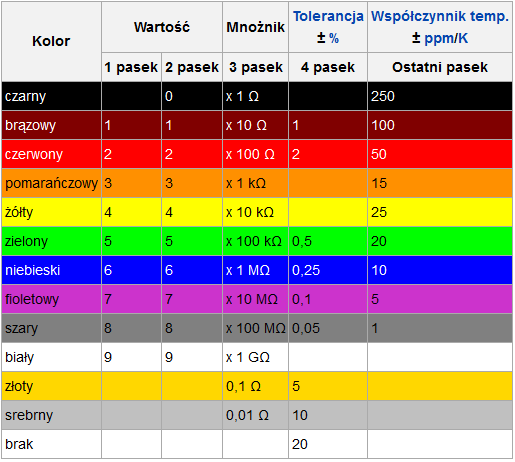
\includegraphics[scale=0.65]{oporniki}
\captionsource{Oznaczenia rezystorów}{\url{https://sites.google.com/site/informatykaunijna/home/poszczegolne-czesci/rezystor}}
\label{fig:oporniki}
\end{figure}
	


	
\begin{wrapfigure}{l}{0.5\textwidth}
\begin{center}
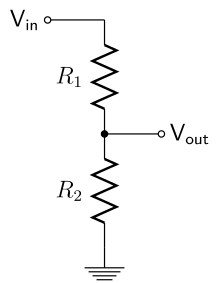
\includegraphics[width=0.48\textwidth]{v-divider}
\captionsource{Układ dzielnika napięcia}{\url{https://www.wikiwand.com/en/Voltage_divider}}
\label{fig:divider}
\end{center}
\end{wrapfigure}
Sposób działania układu, nazywanego dzielnikiem napięcia jest pokazany na rysunku~\ref{fig:divider}, oraz wyraża się wzorem
	$$
		\nu_{out} = \nu_{in}\left[ \frac{R_2}{R_1+R_2}\right]
	$$	
Wzór ten podaje napięcie wyjściowe $\nu_{out}$, które równa się napięciu wejściowemu $\nu_{in}$ przeskalowanemu przez stosunek rezystorów. W opisywanym przypadku jest to stosunek zastosowanego rezystora $4.7 k\Omega$ wyrażonego we wzorze poprzez $R_2$, do sumy tego rezystora wraz z oporem wytwarzanym poprzez czujnik wygięcia $R_1$ - który jak opisano w podrozdziale~\ref{subsec:wygiecie} jest zmienny. Oznacza to że im bardziej czujnik wygięcia jest zgięty, wytwarza on większy opór a co za tym idzie napięcie wyjściowe spada. Miara ta obrazuje jak bardzo palec jest zgięty i jest możliwa do uzyskania właśnie dzięki zastosowaniu układu dzielnika napięcia~\cite{v-divider}.


\section{Budowa rękawicy}
\label{sec:budowa}

W poniższej sekcji zaprezentowano sposób w jaki zostały złączone wszystkie elementy rękawicy wspomniane w sekcji~\ref{sec:przeglad}, aby była gotowa na oprogramowanie mikrokontrolera tworząc finałowy produkt. W tym celu została wybrana rękawica budowlana o grubych niciach ze ściągaczem wokół nadgarstka w celu zapewnienia komfortu, jak i precyzji położenia. Wybór ten również jest uzasadniony faktem początkowego planu dotyczącego wszycia materiału bezpośrednio w rękawice jak i elastyczności które zapewnia grubsza rękawica. Tak jak wspomniano w podsekcji~\ref{subsec:wygiecie}, do połączenia elementów została wykorzystana nić przewodząca. Dzięki grubym włóknom odstępu pomiędzy nićmi przewodzącymi prąd mogły być mniejsze, bez obawy przed spięciami w trakcie poruszania ręką. Dla tego projektu kontroler jest budowany dla lewej dłoni. Układ przewodów kontrolera jest zobrazowany na rysunku~\ref{fig:circuit}. Jest to jedynie obraz poglądowy, przedstawiony na płytce prototypowej a szczegółowy opis połączeń kontrolera zostanie opisany poniżej.

\begin{figure}[h]
\centering
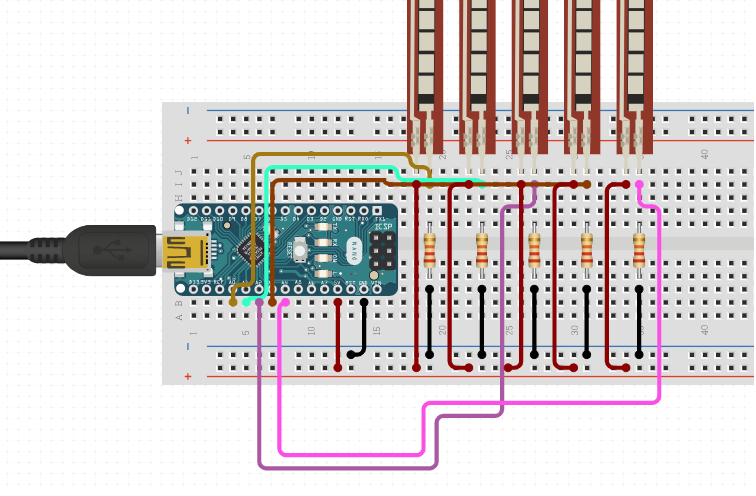
\includegraphics[width=\textwidth]{circuit}
\captionsource{Poglądowy układ kontrolera przedstawiający sposób podłączenia dzielnika napięcia}{\url{https://www.circuito.io/app?components=514,8606,8606,8606,8606,11022}}
\label{fig:circuit}
\end{figure}

\begin{figure}[h]
\centering
%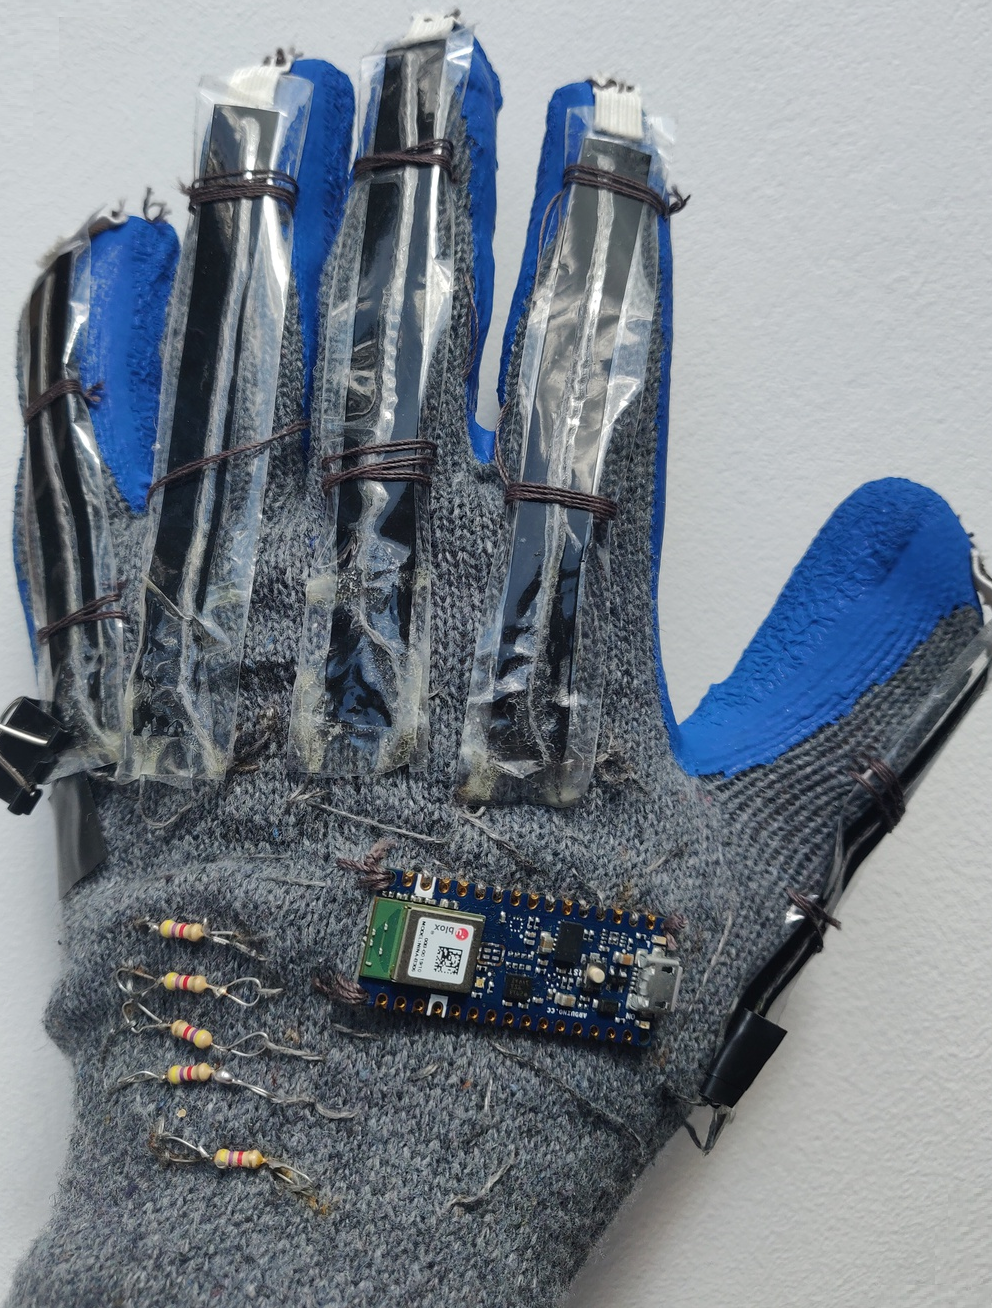
\includegraphics[width=\textwidth]{glove}
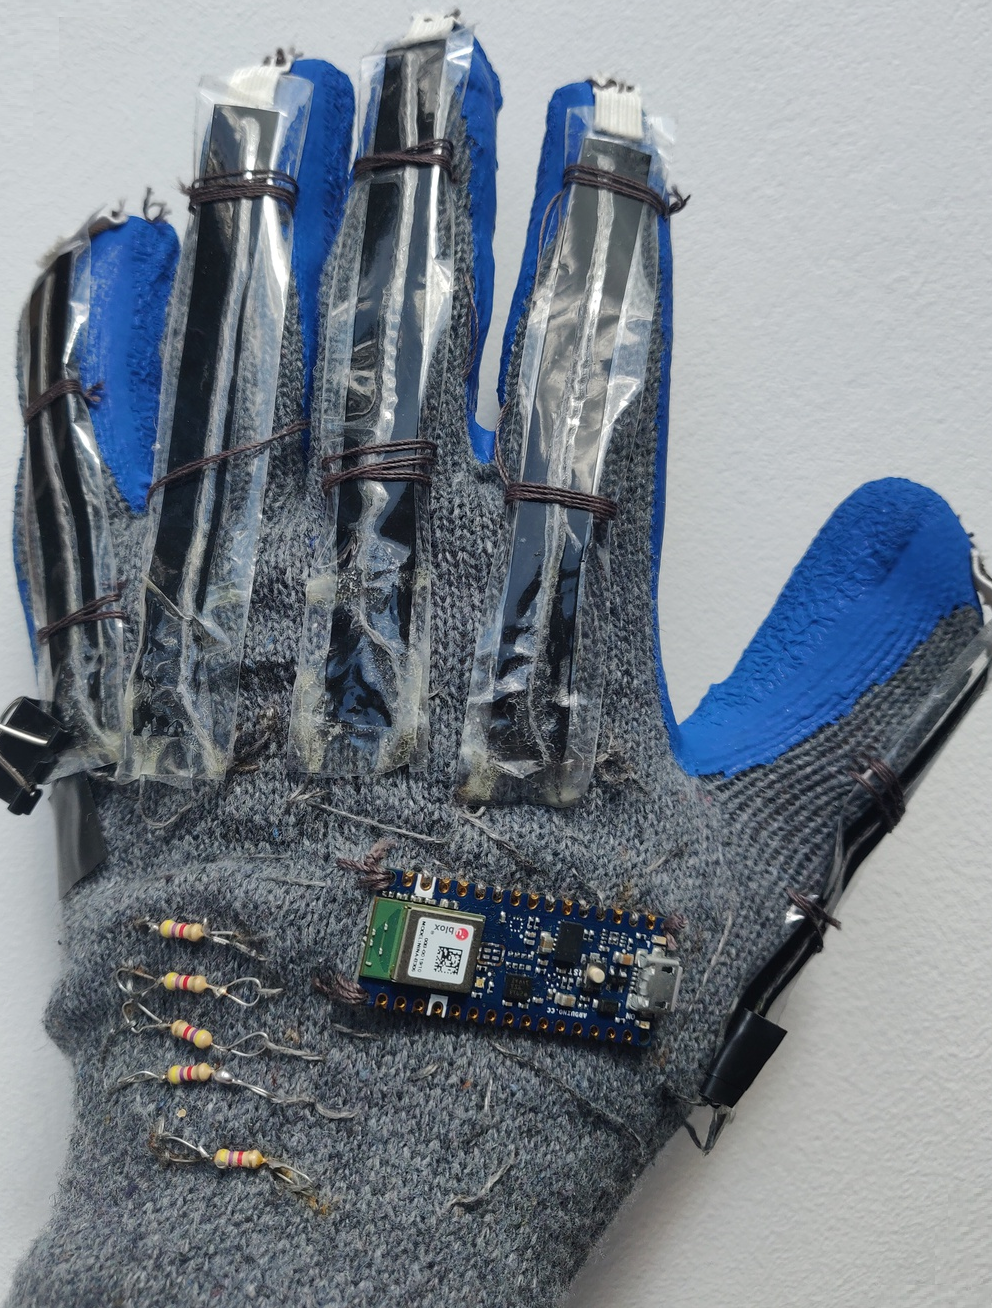
\includegraphics[scale = 0.35]{glove}
\caption{Efekt końcowy rękawicy-kontrolera}
\label{fig:glove}
\end{figure}

Mikroprocesor został umieszczony na wysokości centralnej części dłoni, przy kciuku, skierowany złączem USB na zewnątrz, pozwalając na łatwe podłączenie przewodu zasilającego jak i również ustawienie wejść analogowych w stronę palców lewej dłoni. Z tej strony płytki Arduino będziemy też korzystać - zarówno przy wyprowadzaniu napięcia jak i uziemienia. Montaż samej płytki nie stanowi żadnego problemu ze względy na cztery otwory w rogach pozwalające na mocowanie, do którego została użyta zwykła nić do szycia. Aby stworzyć obwód wychodzący od pinu GND (z ang. Ground) czyli właśnie uziemienia, należy najpierw poprowadzić go przez rezystory. W tym celu wyjścia oporników zostały wygięte w pętle oraz zalutowane aby w łatwy sposób można było je przyszyć do rękawicy. Aby dodatkowo ułatwić sobie to zadanie - dodatkowo zostały one przyklejone bezpośrednio do materiału na bardzo małą ilość kleju. Umiejscowienie rezystorów jest po zewnętrznej wierzchniej stronie dłoni, zaczynając się na wysokości kontrolera, zmierzając szeregowo w stronę nadgarstka. W ten oto sposób nić przewodząca została poprowadzona na zewnętrzną część dłoni a następnie poprzez wszystkie pętle rezystorów, kończąc na ostatnim. Z drugiej strony rezystora dochodzi natomiast nić pochodząca z czujnika oporu. W tym celu podczas tworzenia czujników oporu pozostawiono 25 cm długości nici, co pozwoliło na przymocowanie sensorów, a następnie połączenie obwodu. Sensory zostały zaopatrzone w krótkie, 1-2 cm długości kawałki taśmy elastycznej która została przyklejona na czubku każdego z sensorów pozwalając na elastyczny ruch sensora bez zerwania nici. Taśma ta została przyszyta w czubkach palców co dało punkt zaczepu dla sensorów. W tym momencie pozwoliło to na wygodne używanie nici wychodzących z sensorów w celu zamknięcia obwodu. Z powodu dużego zagęszczenia nici, które nie mogą się ze sobą stykać podczas ruchu ręki, ważnym dla projektu było naprzemienne używanie przestrzeni na rękawicy od spodu jak i od góry. Dzięki temu nici uziemienia oraz napięcia mogą się krzyżować nie zaburzając przy tym odczytów z sensorów. W celu jak najlepszego zagospodarowania przestrzenią wokół sensorów, uziemienie kciuka oraz małego palca zostały umiejscowione na nicie wychodzącej z prawej strony sensora, natomiast napięcie po lewej stronie. Dla pozostałych palców ustawienie to jest odwrotne. Mając to na uwadze została poprowadzona nić od kciuka poprzez wyjście 3.3 V na płytce a następnie wzdłuż knykci rękawicy, pozwalając nicią odpowiedzialnym za napięcie w odpowiednich sensorach na przyczepienie się w celu poboru napięcia tworząc tym samym dodatnią stronę układu. Nici wychodzące z sensorów które natomiast nie zostały do tej pory użyte, zostały przeszyte poprzez wyjścia analogowe a następnie podłączone kolejno do odpowiadających im rezystorów. Wyjścia odpowiadające każdemu z palców zostały opisane w tabeli poniżej. 

\begin{center}
\begin{tabular}{|c|c|}
\hline
Palec & Wyjście analogowe \\ \hline
Kciuk & A3 \\ \hline
Wskazujący & A0 \\ \hline
Środkowy & A1 \\ \hline
Serdeczny & A6 \\ \hline
Mały & A7 \\ \hline
\hline
\end{tabular}
\end{center}

Sposób w jaki zostały dobrane wyjścia jest podyktowany zaleceniami o nie korzystaniu z wyjść analogowych A4 oraz A5 oraz pozostawieniu przestrzeni wokół wyjścia A3 przeznaczonego na kciuka, ponieważ jako jedyne połączenie musiało najpierw zmierzać w kierunku palców a następnie w dół w celu połączenia z rezystorem. Efekt końcowy pracy przedstawia zdjęcie~\ref{fig:glove}.

\section{Oprogramowanie mikrokontrolera}
\label{sec:oprogramowanie}


Do tej pory została opisana teoria omawianego kontrolera, elementy które zostały użyte w projekcie a także sposób ich połączenia. W niniejszej sekcji przedstawiony jest kod programu który został napisany w środowisku programistycznym oraz języku o tej samej nazwie - Arduino. Język ten poza drobnymi zmianami opiera się na języku C/C++, a jego pełny kod źródłowy jest dostępny na platformie Github~\cite{jArduino}. Aby rozpocząć pracę z wybranym produktem od Arduino należy wykonać pewne czynności przygotowywacze, takie jak instalacja sterowników płytki dla danego systemu czy sposób obsługi w samym środowisku Arduino. Czynności te zostały opisane na stronie producenta, w związku z czym nie zostaną one szczegółowo opisane~\cite{guideArduino}. Po spełnieniu wszystkich wymagań, został przygotowany program który został napisany oraz wgrany do mikrokontrolera, który można podzielić na trzy części:
\begin{itemize}
\item Deklaracje
\item Ustawienie mikrokotrnolera
\item Główna pętla programu
\end{itemize}
których cel oraz opis został przedstawiony poniżej.

W pierwszej kolejności zostanie przedstawiona część deklaracji, w której to dołączono wymagane biblioteki dla poprawnej obsługi wszystkich sensorów. Pierwszą biblioteką która została dołączona do programu jest \textit{Arduino\textunderscore LSM9DS1.h}. Biblioteka ta jest odpowiedzialna za obsługę IMU która przekazuje dane poprzez I2C do mikroprocesora. Biblioteka ta zajmuję się obsługą połączenia jak i kalibracja całego modułu. Inicjalizacja wartości poprzez biblitoekę wygląda w następujący sposób~\cite{ArduinoIMU}
\begin{center}
\begin{tabular}{|c|c|c|}
\hline
Sensor & Zakres & Częstotliwość \\ \hline
Akcelerometr & $[-4,+4]g -/+0.122 mg$ & $104 Hz$\\ \hline
Żyroskop & $[-2000, +2000] dps +/-70 mdps$ & $104 Hz$\\ \hline
Magnetometr & $[-400, +400] uT +/-0.014 uT$ & $20 Hz$ \\ \hline
\hline
\end{tabular}
\end{center}
Tak jak wspomniano w sekcji~\ref{subsec:arduino} do połączenia bezprzewodowego Arduino Nano 33 BLE wykorzystuje moduł Bluetooth Low Energy, w związku z czym w części deklaracji dołączamy przeznaczoną do tego bibliotekę o nazwie \textit{ArduinoBLE.h}. Biblioteka ta pozwala na dostęp oraz sterowanie modułem BLE ( z ang. Bluetooth Low Energy), i na potrzeby projektu zostaną opisane używane elementy z poniższych klasy których znajomość jest wymagana w celu zrozumienia napisanego programu. Klasy te to
\begin{itemize}
\item BLEService
\item BLECharacteristic
\item BLEDescriptor
\item BLE
\item BLEDevice
\end{itemize}
Szczegóły na temat zasad działania BLE są podane w sekcji~\ref{sec:bvsble}, w tej sekcji jedynie zostanie opisana struktura tych klas. \textit{BLEService} umożliwia nawiązanie połączenia z innym urządzeniem obsługującym bluetooth i jako parametr przyjmuje UUID - jest to jedyny paramater jaki należy podać i w ten sposób zostaje stworzony nowy serwis BLE dostępny pod tym identyfikatorem. Klasa \textit{BLECharacteristic} tworzy nową cechę którą należy przypisać do danego serwisu. Cecha ta może zostać zadeklarowana jako cecha wybranego z pośród dostępnych typów w Arduino bądź jako uniwersalna poprzez podstawową klasę \textit{BLECharacteristic}. Klasa ta przyjmuje trzy wymagane parametry: UUID, właściwości cechy oraz wartość. Wartość może zostać zadeklarowana jako podany ciąg znaków, bądź też poprzez określenie rozmiaru danych i wartość początkową. Wartość początkowa nie musi być podana w trakcie deklaracji. Ważnym elementem tej klasy jest określenie jej właściwości. W zależności od przeznaczenia mamy do wybory następujące opcje, które mogą być ze sobą łączone: BLEBroadcast, BLERead, BLEWriteWithoutResponse, BLEWrite, BLENotify, BLEIndicate. W celu wysyłania danych podczas gdy dane te się zmienią cechy w prezentowanym programie przyjęły dwie wartości BLE: read ( z ang. czytać) oraz notify (z ang. powiadomić). Klasa \textit{BLEDescriptor} jest niejako klasą pomocniczną. Wartości tej klasy przypisuję się do danej cechy w celu lepszej obsługi serwisy oraz łatwiejszego rozpoznawania w przypadku pracy ze skomplikowanymi serwisami. Standardowo należy podać UUID danego deskryptora jako parametr, a także jego wartość jako ciąg znaków, bądź wartość w postaci tablicy bajtów oraz maksymalnego rozmiaru danych. Są to podstawowe klasy znajdujące się w części deklaracji których użycie zostały przedstawione na listingu~\ref{lst:declaration} prezentującym wycinek części deklaracji~\cite{ArduinoBLE}. Pozostałe dwie klasy zostaną opisane w części głównej pętli programu gdzie zostanie również pokazane ich zastosowanie. \newpage 

\begin{lstlisting}[caption={Część deklaracji programu mikrokontrolera},captionpos=b,label={lst:declaration},language = C++ , frame = trBL , firstnumber = last , escapeinside={(*@}{@*)}]
#include <Arduino_LSM9DS1.h>
#include <ArduinoBLE.h>
BLEService imuService("1101");

BLECharacteristic imuAccChar("2101", BLERead | BLENotify,12);
BLECharacteristic imuGyroChar("2102", BLERead | BLENotify, 12);
BLECharacteristic fingersChar("2103", BLERead | BLENotify, 20);

BLEDescriptor     imuAccDescriptor("3101",(byte*)"Acc Descriptor",15);
BLEDescriptor     imuGyroDescriptor("3102",(byte*)"Gyr Descriptor",15);
BLEDescriptor     fingersDescriptor("3103",(byte*)"Fin Descriptor",15);
\end{lstlisting}

Następną częścią programu jest ustawienie mikrokontrolera oraz sprawdzenia poprawności działania sensorów. Gdy proces ten zakończy się powodzeniem zostanie uruchomiona główna część programu - funkcja \textit{loop()}, która wykonuję się nieprzerwania pozwalając kontrolować pracę naszego kontrolera. Za część związaną z inicjalizacją jest odpowiedzialna funkcja \textit{setup()}. Funkcja ta jest wywoływana tylko raz za każdym razem gdy płytka jest podłączona do prądu bądź zostanie zresetowana~\cite{ArduinoDoc}. W funkcji tej wywoływana jest statyczna metoda begin(z ang. rozpocząć) na klasie \textit{IMU} która należy do biblioteki \textit{Arduino\textunderscore LSM9DS1.h}, i to właśnie ta funkcja pozwala na incjalizacje wspominanych sensorów wchodzących w skład jednostki pomiarowej - program zapętli się w tym miejscu jeśli funkcja ta zwróci błąd, poprzez rozpoczęcie pętli z warunkiem zawsze prawdziwym, co przedstawia listing~\ref{lst:init}~\cite{ArduinoIMU}. 
\begin{lstlisting}[caption={Inicjalizacja IMU oraz BLE},captionpos=b,label={lst:init},language = C++ , frame = trBL , firstnumber = last , escapeinside={(*@}{@*)}]
  if (!IMU.begin()) {
    Serial.println("Failed to initialize IMU!");
    while (1);
  }

  if (!BLE.begin()) {
    Serial.println("Failed to start Bluetooth!");
    while (1);
  }
\end{lstlisting}
Jeżeli sensory działają poprawnie, sprawdzana jest możliwość połączenia poprzez moduł bezprzewodowy. W tym celu wykorzystywana jest statyczna klasa \textit{BLE}, która odpowiada za włączenie modułu Bluetooth oraz jego ustawienia. Tak jak w przypadku klasy \textit{IMU}, program zapętli się w tym miejscu zwracając błąd jeżeli połączenie nie będzie możliwe. W przypadku powodzenia program rozpoczyna łączenie zadeklarowanych elementów, takich jak serwis, cechy oraz deskryptory tych cech. Klasa \textit{BLE} posiada funkcje pozwalającą ustawić nazwę dla naszego połączenia, jej adres a przede wszystkim gdy wszystkie elementy są już gotowe wywołuję metodę \textit{advertise()}, która pozwala na połączenie się z naszym serwisem. Na listingu~\ref{lst:initBle} pokazane jest szczegółowa konfiguracja klasy BLE oraz serwisu a także odpowiednie użycie funkcji dla jednej z cech, które należy powtórzyć dla każdej dodawanej cechy z odpowiednimi wartościami.
\begin{lstlisting}[caption={Obsługa serwisu przy użycia klasy BLE},captionpos=b,label={lst:initBle},language = C++ , frame = trBL , firstnumber = last , escapeinside={(*@}{@*)}]
  BLE.setLocalName("VrGlove");  
  BLE.setAdvertisedService(imuService);

  imuService.addCharacteristic(imuGyroChar);
  imuGyroChar.addDescriptor(imuGyroDescriptor);
  imuGyroChar.writeValue((byte)0x01);
  
  BLE.addService(imuService);     
  BLE.advertise();
\end{lstlisting}
W ten oto sposób kończy się funkcja \textit{setup()} i zostaje wywołana kolejna funkcja która od tej pory będzie odpowiedzialna za pracę kontrolera - \textit{loop()}. W funkcji tej zostaje zadeklarowana ostatnia z wymienionych klas do obsługi Bluetooth. Klasa ta nazywa się \textit{BLEDevice} i jest bezpośrednio powiązana z urządzeniem które jest aktualnie podłączone. Dopóki nie ma podłączonego do kontrolera urządzenia, żadne czynności nie zostają podjęte. W momencie uzyskania danych z modułu łączności o nawiązanym połączeniu zostaje uruchomiona pętla, funkcjonująca tak długo jak połączenie to nie zostanie przerwane. Fragment kodu znajduję się na listingu~\ref{lst:central}~\cite{ArduinoBLE}. Niestety w trakcie pracy z urządzeniem odkryto błąd związany z rozłączeniem się centrali. Problem pojawia się gdy urządzenie zostaję rozłączone z mikrokontrolerem - w tym momencie klasa \textit{BLE} nie zawsze zgłasza informację o rozłączeniu, myśląc że urządzenia cały czas są podłączone. Problem został zauważony, jednak nie jest rozwiązany na stan z maja 2020 roku~\cite{ArduinoBug}. 
\begin{lstlisting}[caption={Oczekiwanie na połączenie z urządzeniem przez mikrokontroler},captionpos=b,label={lst:central},language = C++ , frame = trBL , firstnumber = last , escapeinside={(*@}{@*)}]
  BLEDevice central = BLE.central();
  if (central) {
    Serial.print("Connected to central: ");
    Serial.println(central.address());
  }  
   while( central.connected()){ 
   		[...]
   	}
\end{lstlisting}
Gdy wszystkie dotychczasowo opisane elementy programu nie zgłoszą problemów, następuje ostatnia faza którą jest zbieranie i przesyłanie danych. W pierwszej kolejności sprawdzany jest warunek czy jednostka pomiarowa ma dostęp do nowych danych. W przypadku tej aplikacji dane które zostały poddane analizie pochodzą z żyroskopu oraz z akcelerometru i są wyrażone jako zmienne x,y oraz z typu \textit{float}. Z powodu naturalnych drgań dłoni dane te ciągle się zmieniają w mikro skali która nie ma wpływu na efekty, niemniej jednak możemy założyć że gdy mikroprocesor nie jest przymocowany do stałego obiektu, dane te będą dostarczane z częstotliwością pracy sensorów. Za odczyt danych z żyroskopu i akcelerometru odpowiadają odpowiednio funkcje \textit{readGyroscope(x,y,z)} oraz \textit{readAcceleration(x,y,z)} z klasy \textit{IMU} które przypisuję odpowiednie wartości do podanych parametrów. Ważnym elementem podczas odczytu tych danych jest tak zwany szum który powstaje w trakcie przygotowania sensorów. W trakcie pierwszych odczytów szum ten został zmierzony oraz usunięty z pomiarów. Akcelerometr położony na płaskim obiekcie prawidłowo podawał odczyty, czyli zwracał wektor $[0,0,g]$ gdzie \textit{g} oznacza grawitacje ziemską. Żyroskop natomiast wskazywał błąd rzędu $[2.80,0.18,0.18]$ w związku  z czym od każdego odczytu właśnie taką wartość należy odjąć w celu uzyskania prawidłowych danych - czyli wektora zbliżonego do $[0,0,0]$ w pozycji w której został skalibrowany. Jak wspomniano w sekcji~\ref{subsec:sensory} dotyczącej żyroskopu, wartości zwracane są podane w $\frac{rad}{s}$, również znane jako dps (z ang. Degrees per second) czyli w kątach na sekundę. W celu określenie kątów w jakim urządzenie się znajduję w danym momencie musimy te dane przemnożyć przez częstotliwość z jaką są one pobierane - czyli przemnożyć przez czas co zwróci nam miarę kątów. Osiągamy to poprzez zapisanie czasu w którym dane zostały pobrane a także poprzez zapisanie tej wartości przed następnym pobraniem danych jako czas ostatniego poboru. Różnica pomiędzy tymi wartościami daje czas jaki upłynął aby uzyskać nowe wartości. Zaczynając w pozycji kalibracyjnej, z idealnie usuniętym szumem, żyroskop zwróci wartość zero, a wraz ze zmianą wartości żyroskopu, suma tych zmian wskaże na orientację kontrolera względem pozycji wyjściowej. Więcej informacji na ten temat znajduję się w rozdziale~\ref{ch:aplikacja}~\cite{gimbal}. Ostatnią cechą którą chcemy przekazać są dane pobierane z sensorów wygięcia w celu określenia pozycji palców. Tak jak wspomniano w sekcji~\ref{sec:przeglad} dane te pobieramy przez mierzenie napięcia jakie znajduje się na poszczególny analogowych pinach wejściowych. Odczyty te uzyskujemy poprzez wywołanie metody \textit{analogRead(pin)}~\cite{ArduinoDoc}. Pobieranie danych oraz ich wstępna obróbka przedstawia listing~\ref{lst:read}. \newpage
\begin{lstlisting}[caption={Wczytywanie danych z sensorów.},captionpos=b,label={lst:read},language = C++ , frame = trBL , firstnumber = last , escapeinside={(*@}{@*)}]
 if (IMU.accelerationAvailable() && IMU.gyroscopeAvailable()) {
        previousTime = currentTime;
        currentTime = millis();
        elapsedTime = (currentTime - previousTime) / 1000;   

        IMU.readAcceleration(acc[0],acc[1], acc[2]);  
        IMU.readGyroscope(gyro[0],gyro[1], gyro[2]);
        
        gyro[0] -= 2.80;
        gyro[1] -= 0.18;
        gyro[2] -= 0.18;

        fingers[0] = analogRead(A3);
        [...]
 }
\end{lstlisting}
Na tym etapie mamy już dostęp do danych z akcelerometru w {\Large $\frac{m}{s^2}$} oraz dane z żyroskopu wyrażone w stopniach. Informacje te mogłyby zostać przesłane w takiej formie, jednak z racji znajomości projektu, dane można dodatkowo skorygować poprzez zastosowanie dodatkowych filtrów. Podstawowym zabiegiem który został zastosowany jest eliminacja danych nieznaczących, czyli szumu który powstaje poprzez naturalne drgania ciała. Aby to osiągnąć, w programie przechowywane są poprzednie wartości z poszczególnych sensorów. Jak dane znaczące dla akcelerometru przyjęto różnice $\pm 0.1$, a dla danych z sensorów wygięcia $\pm 15$. Dla żyroskopu natomiast przyjęto wartości różniące się o przynajmniej $\pm 0.2$, a także dodatkowo sprawdzane jest czy dane z żyroskopu nie są w pozycji przy kalibracyjnej. Oznacza to że jeżeli wartości zwracane z żyroskopu wynoszą $0\pm 0.1$, zostaną one zamienione na wartość równą $0$. Filtrowanie wartości pokazane jest na listingu~\ref{lst:filtr}. W ten oto sposób otrzymano wartości z sensorów które były gotowe do wysłania na inne urządzenie. Wartości te jednak są wyrażone w postaci tablic typu \textit{float}, natomiast jako wartości cechy bluetooth przyjmują tablice bytów. W związku z tym przed przypisaniem danych są przekazywane adresy tablic do nowych zmiennych, a następnie zmienne te zapisane w poszczególnej cesze przy użyciu metody \textit{setValue(value,valueSize)}. Rozmiar jest ten określony jako $12$ ponieważ mamy do czynienia z tablicą 3 zmiennych typu \textit{float} z których każda zajmuje 4 bajty pamięci. Zapisywanie danych jest pokazana na listingu~\ref{lst:save} dla jednej cechy - proces ten należy powtórzyć dla wszystkich danych. Program następnie zapisuje obecne dane jako dane obecnej pętli, tak aby następne odczyty mogły zostać porównane z obecną iteracją, tym samym kończąc wykonywaną pętle. Warto zauważyć że program pomimo swojego głównego działa w funkcji \textit{loop()}, jest wykonywany w ramach jednej iteracji jak tylko dojdzie do połączenia kontrolera z odbiornikiem.
\begin{lstlisting}[caption={Wstępne filtrowanie danych z sensorów.},captionpos=b,label={lst:filtr},language = C++ , frame = trBL , firstnumber = last , escapeinside={(*@}{@*)}]
for (int i = 0;i<3;i++){
	if(!(gyro[i] < oldGyroData[i]-0.2 || gyro[i] > oldGyroData[i]+0.2)){
		if( gyro[i] < -0.1 ||  gyro[i] > 0.1){              
	      gyro[i] = oldGyroData[i];
	    }else{
	     gyro[i] = 0.0;
	    }
	}
	            
	if(!(acc[i] < oldAccData[i]-0.02 || acc[i] > oldAccData[i]+0.02)){
	   acc[i] = oldAccData[i];
	   }
}

for (int i = 0;i<5;i++){
   if(!(fingers[i] < oldFingersData[i]-15.0 || fingers[i] > oldFingersData[i]+15.0)){
              fingers[i] = oldFingersData[i];
            }
         }         
 }
\end{lstlisting}

\begin{lstlisting}[caption={Zapisywanie danych do cech w serwisie.},captionpos=b,label={lst:save},language = C++ , frame = trBL , firstnumber = last , escapeinside={(*@}{@*)}]
         byte *accChar = (byte*)&acc;
         imuAccChar.setValue(accChar,12);
\end{lstlisting}

\section{Dalszy rozwój}
\label{sec:rozwoj}
\improvement{Przypis z pracy dla wszystkich podrzodziałów}
\improvement{Wykorzystania projketu pokazano w drugiej pracy}
 W rozdziałach~\ref{ch:rekawica} i~\ref{ch:aplikacja} pokazano budowę kontrolera oraz aplikacji która wykorzystuje zbudowany kontroler w celu obsługi podstawowych funkcji rękawicy-kontrolera. Projekt ten powstał z myślą ograniczonego budżetu, prostoty wykonania oraz możliwości replikacji. Założenia te spowodowały że zdecydowano się na pewne rozwiązania które w końcowej wersji projektu pokazały swoje wady. W tym rozdziale zostanie poruszony temat błędów popełnionych w pierwszej wersji tego projektu oraz przykładowe sposoby na ich rozwiązanie w przyszłości. 
 
 \subsection{Problemy mikroprocesora}
 \label{subsec:iuMikroprocesor}
 Przede wszystkim szukano małego mikrokontrolera tak aby nie był on przeszkodą podczas użytkowania kontrolera. O ile założenie to było dobrym pomysłem, okazało się że umiejscowienie przy brzegu sprawiło że ruch palców, w szczególności kciuka, może zmienić położenie jednostki IMU na rękawicy. Oznacza to że nawet jeśli nasza ręka znajduję się w stałej pozycji, samo poruszanie palcami wprowadza błąd w odczycie. Niestety wybór tego produktu od Arduino również przysporzył wiele kłopotów z racji błędnego rozłączania się adaptera Bluetooth. Z dotychczasowego użytkowania można stwierdzić iż kontroler poprawnie łączy się i rozłącza dwa razy, zaś w większości testowanych przypadków dochodzi do błędu połączenia przy trzeciej próbie. Aby usunąć ten błąd należy odłączyć płytkę od zasilania i podłączyć ponownie, resetując tym samym moduł. Samo oprogramowanie rękawicy skupia się na odczytach z dwóch sensorów. Praktyka pokazała że dane te nie są wystarczająco dokładne, i jeżeli to możliwe powinny być pobierane również dane magnetometru w celu dodatkowego korygowania odczytów z żyroskopu. 
 
 \subsection{Problemy budowy i czujników wygięcia}
 \label{subsec:iuPalce}
 Problem z użytkowaniem rękawicy pojawił się dość szybko od jej zbudowania. Mianowicie wybrana do projektu rękawica była zbyt gruba, powodując dyskomfort w użytkowaniu w szczególności przez dłuższy okres czasu. Początkowe kryterium elastyczności, przesądziło o wybraniu tej rękawicy, jednak cienka rękawica również spełniła by wymagania końcowego produktu. Rozwiązanie zastosowane w celu odczytu wygięcia palców z założenia wyglądało na idealnie pasujące do wymagań projektu. Pomimo swojej prostoty wykonania oraz braku pomiaru takich cech jak odwodzenie palców czy też wygięcie poszczególnych stawów, spełnia ono swoją podstawową funkcję. Problemem tego rozwiązania jest natomiast brak elastyczności sensorów. W momencie zgięcia palców droga od knykci do paznokci się wydłuża sprawiając że sensor jest poddawany sile nacisku od strony palca która jest tym spowodowana. Sensory te pomimo braku elastyczności są zbudowane z materiału wytrzymałego na rozciąganie dzięki czemu nie pękają podczas zgięciu palców, jednak w celu zapewnienia lepszego mocowania i większej ochrony, z jednej strony została przymocowana elastyczna guma która trzyma sensor przy czubkach palców, z drugiej natomiast sensor został wszyty w rękawicę. Problem który się pojawił w trakcie użytkowania pochodził ze sposobu wszycia sensora. Została do tego użyta nić przewodząca która z powodu rozciągliwości rękawicy nie mogła zostać wszyta na sztywno, w związku z czym stawiała ona mniejszy opór podczas zginania palców i niejako została wyciągnięta przez sensor, powodując tym brak dokładności odczytów. Nić ta oprócz niskiej elastyczności okazała się być nietrwała. W trakcie korzystania z rękawicy doszło do kilku pęknięć, które zostały ponownie związane, jednak została przerwana w ten sposób ciągłość obwodu. Przez dodanie dodatkowych wiązań odczyty z sensorów się pogorszyły, sprawiając że wygięcie palca wskazującego ma większy wpływ na odczyty z kciuka, niż zgięcie kciuka samo w sobie. Podobna sytuacja przytrafiła się z sensorem małego palca oraz serdecznego. Mała powierzchnia na dłoni wokół której należało poprawić wiele połączeń, sprawiła że część nici była blisko siebie, powodując momentami odczuwalne mrowienie na dłoni. Problem ten został rozwiązany poprzez zastosowanie izolacji od wewnętrznej strony rękawicy, jednak nie gwarantuje to przeciwdziałaniu zwarć w obwodzie. Konkludując, nić przewodząca nie jest najlepszym rozwiązaniem w celu połączenia elementów dla tego projektu i powinno zostać zastąpiona trwalszym połączeniem. Gdyby jednak została ona użyta, element przewodzący powinien znajdować się w środku oplotu, bądź powinny zostać zastosowane inne sposoby izolacji, a sama wytrzymałość nici powinna być znacznie większa. Mocowanie sensorów wygięcia powinno być bardziej trwałe oraz statyczne, nie pozwalając na przemieszczenie sensora na palcu. Alternatywą dla tego rozwiązania jest wykorzystanie czujników pomiaru wygięcia opartych o światło nadawane z jednej strony plastikowej tuby oraz miernika natężenia światła z drugiej. W ten sposób wiadomo że im mniejszy pomiar otrzymywanego światła, tym większe wygięcie tuby, której załamanie blokuje bezproblemowy dopływ światła. Rozwiązanie to również zapewnia pomiary niezniekształcone poprzez zachowanie innych sensorów a także wygląda na bardziej dokładne~\cite{ledsensor}.
 
 
  \subsection{Animacja modelu}
 \label{subsec:iuAnimacja}
 Ostatnim elementem aplikacji dla projektu jest zapewnienie animacji dłoni. W tym celu został wykorzystany \textit{Google Sceneform}, dzięki któremu zaimportowano modele, ustawiono scenę, przypisano model a także obsługiwano przemieszczenie i orientację. Ostatnim brakującym elementem jest animacja modelu. Według dokumentacji starszej wersji projektu osiągnąć to można poprzez klasę \textit{SkeletonNode}, pozwalającą na dostęp do kości modelu, bez wykorzystania zewnętrznego programu graficznego. Jednak z niejasnych przyczyn klasa ta została usunięta w ostatniej wersji SDK, powodując brak możliwości wprowadzania zmian w modelu który został zaimportowany przy użyciu wtyczki. Problem ten rozwiązano poprzez wykorzystanie programu \textit{Blender}, dzięki któremu można było wyeksportować modele w wyznaczonej pozycji. Aby osiągnąć jednak animację modelu w czasie rzeczywistym, na podstawie dostępnych danych z sensorów wygięcia - cała klasa renderująca fragment~\ref{fig:ifceAnimacja} musi zostać napisana od nowa z wykorzystaniem innej technologii, ponieważ na oficjalnej stronie dystrybucji \textit{Sceneform}, jest napisane iż projekt został zarchiwizowany, w związku z czym taka opcja nie zostanie dodana~\cite{sceneform}. 
 
  \subsection{Błąd rotacji}
 \label{subsec:iuRotacja}
 W przypadku rotacji jest wiele sposobów na polepszenie rezultatów. W prezentowanym projekcie wybrano podstawową metodę która wykorzystuje jedynie żyroskop oraz akcelerometr i przy ich użyciu wykorzystuje filtr komplementarny. Tak jak wcześniej wspomniano, aby dokładnie skorygować żyroskop na wszystkich trzech osiach, należy wykorzystać również magnetometr. Oprócz tego istnieje wiele filtrów takich jak Kalmana czy Madgwick'a które skutecznie usuwają szum, a także algorytmy wykorzystujące nowe pomiary w połączeniu z tymi zebranymi przed nimi. Możliwości łączenia technik udoskonalania odczytu rotacji z jednostek IMU sprawia, że nie ma jednego najlepszego rozwiązania, a ich wybór jest uzależniony on rodzaju projektu nad którym się pracuje~\cite{sensorslab}. 
 
 
 \subsection{Problem obliczania przesunięcia}
 \label{subsec:iuPrzesunięcie}
 Obliczenie położenia kontrolera w przestrzeni, niewątpliwie należy do najtrudniejszego problemu w tym projekcie. Sedno problemu tkwi w niedokładności danych. Z powodu wykorzystania metody podwójnego całkowania, błąd uzyskiwany w cm przy pojedynczej całce, rośnie do m przy całkowaniu podwójnym. Ekran aplikacji jest mierzony w m, a ruch dłoni z kontrolerem ma ograniczony zasięg długości ramienia. Pomimo tego w niedużym czasie błąd rośnie do poziomu w którym model znika z ekranu użytkownika. Niestety nie istnieje łatwy sposób na skorygowanie błędów powstałych w wyniku tego algorytmu. Firmy zajmujące tym się tym problemem dodatkowo umieszczają czujniki pozwalające określić odbiornik urządzenia i ustalić pozycję względem niego, kamery zewnętrzne obserwujące ruch w przestrzeni a także dodatkowe czujniki optyczne. W przypadku rękawicy-kontrolera który może poruszać się we wszystkich kierunkach dodatkowy problem stanowi rotacja, przez którą błąd staję się coraz większy. W przypadku prostej aplikacji nie wykorzystującej zaawansowanych jednostek pomiarowych oraz algorytmów filtrujących, często efekt jaki można osiągnąć tą techniką nie sprawdza się w zastosowaniu, dlatego też dla tej aplikacji domyślnie funkcja ta jest wyłączona~\cite{sensorslab}. 
 
\section{Podsumowanie projektu}
\label{sec:summary}
W tym rozdziale podano informacje na temat projektu rękawicy kontrolera a także elementów które są wymagane w celu jego funkcjonowania. Zostały podane specyfikacje podzespołów, sposoby pozyskiwania danych, metoda komunikacji z innymi urządzeniami a także rozwiązano problemy związane z kosztem projektu. Krok po kroku przedstawiono złożenie elementów w celu uzyskania końcowej wersji produktu i ostatecznie omówiono zasadę działania programu napisanego w Arduino wraz z bibliotekami które zostały użyte w ramach projektu, natomiast zasady ich praktycznego działania zostały pokazane na listingach. W ten oto sposób została zakończona główna część projektu, pozwalająca na wykorzystanie rękawicy kontrolera jako część większych przedsięwzięć. Aby jeszcze lepiej zobrazować sposób obsługi kontrolera, oraz metody wykorzystania danych, w rozdziale~\ref{ch:aplikacja} zostanie pokazana przykładowa aplikacja wykorzystująca dane w celu analizy oraz prezentacji. 
\chapter*{Podsumowanie}
\label{ch:podsumowanie}
\addcontentsline{toc}{chapter}{Podsumowanie}
Przedmiotem działań podjętych w celu stworzenia tej pracy było stworzenie podstawowej wersji kontrolera którego można używać w sposób intuicyjny poprzez samo poruszanie dłonią, w szczególności przeznaczonych do środowisk wirtualnej rzeczywistości. Projekt miał za zadanie przygotowanie podłoża dla dalszych prac, usprawnień a także poznania przykładowych rozwiązań znajdujących się na rynku. Podjęto działanie w celu zrozumienia problemów oraz rozwiązań nawigacji inercyjnej przy użyciu IMU, poznając zasady działania sensorów które jednostka ta obsługuje oraz standardu przesyłania tych danych poprzez adapter Bluetooth Low Energy. Został również zaadresowany problem pomiaru wygięcia palców przy niewielkim budżecie. Wszystkie te elementy zostały złożone w całość tworząc w pełni sprawny kontroler, zdolny do realizacji przedstawionych celów. Kontroler ten niestety ma też wiele wad które sprawiają że wymaga on wielu usprawnień w przyszłości. W celu poznania metod obsługi kontrolera została napisana aplikacja na system Android, pozwalająca wykorzystać stworzone urządzenie w praktyce. Wykorzystując SDK \textit{Sceneform} została przedstawiony model dłoni, reagujący na działanie kontrolera. Dedykowana aplikacja prezentuje wizualną wersję problemów nawigacji inercyjnej, pokazując skalę problemów które trzeba rozwiązać aby osiągnąć satysfakcjonujące efekty. Dzięki zebranym danym, ustalono błędy wykonane w projekcie oraz przedstawiono przykładowe sposoby na ich rozwiązanie bądź usprawnienie.  

Projekt ten pozwolił na wyciągnięcie wielu cennych lekcji dzięki zrozumieniu wszystkich jego elementów. Dzięki temu można stwierdzić że jest on niejako prototypem docelowego projektu, któremu należy poświęcić dużo więcej pracy. Mając jednak do dyspozycji odpowiednie narzędzia i budżet można osiągnąć satysfakcjonujące rozwiązanie nawet w domowych warunkach w szczególności jeżeli  poruszanym tematem jest orientacja a także kształt dłoni w czasie rzeczywistym. W celu osiągnięcia dokładnego położenia, najlepszym rozwiązaniem pozostaje jak dotąd użycie zewnętrznego systemu do śledzenia położenia. Jeżeli chcemy skorzystać z tego projektu przy użyciu dostępnych na rynku okularów VR, które posiadają w zestawie system namierzania kontrolerów, należałoby jako dodatkowy element zapewnić synchronizację, tworząc tym samym kompletny produkt w domowych warunkach. Jest to niewątpliwie projekt o dużym potencjale, z wciąż rosnącym rynkiem oraz zapotrzebowaniem i zainteresowaniem na tego typu produkty pokazywanym przez wielkie koncerny samochodowe a nawet agencje kosmiczne. Na zakończenie warto dodać że wciąż nie odkryto pełnych możliwości wirtualnej rzeczywistości, co sprawia że praca nad tym projektem jest tak ekscytująca, a na przykładzie tego projektu pokazano że nie jest to ekskluzywny rynek i każdy może w nim wziąć udział w celu zbudowania lepszej i być może wirtualnej przyszłości.  
%
%
\addcontentsline{toc}{chapter}{Bibliografia}
%
\bibliographystyle{abbrv}
\bibliography{bibliografia}
%   
\listoffigures
%
\listoftodos[TODOs:]
%
\end{document}